%\RequirePackage{atbegshi}
\documentclass[10pt]{beamer}

\usetheme{default}
\usepackage{amssymb}
\usepackage{biblatex}
%\usepackage[cmex10]{amsmath}
\usepackage{stmaryrd,epsfig}
\usepackage[english]{babel}
\usepackage{tikz,pgf,pgfplots}
\pgfplotsset{compat=newest}
\usepgflibrary{shapes}
\usetikzlibrary{%
  arrows,%
  decorations,%decorations
  shapes.misc,% wg. rounded rectangle
  shapes.arrows,%
  shapes.callouts, %
  shapes,%
  shadows,%
  shadows.blur,%
  chains,%
  matrix,%
  positioning,% wg. " of "
  patterns,% slanted lines fill
  scopes,patterns,calc,
decorations.markings,
decorations.pathmorphing
}


\makeatletter
\def\myfootnote{\xdef\@thefnmark{}\@footnotetext}
\makeatother

%\setbeamertemplate{blocks}[rounded][shadow=true]

% Radius of regular polygons
\newdimen\R
\R=0.8cm

\definecolor{tutorial}{RGB}{50,93,61}


\title{Leveraging Structural Properties of Tree Coding\\
in AMP for the Unsourced MAC}
\author{J.-F.~Chamberland \newline
\textcolor{gray}{Vamsi K. Amalladinne, Asit Kumar Pradhan,\\
Cynthia Rush$^\dagger$, Krishna R. Narayanan}}
\institute{Electrical and Computer Engineering @ Texas A\&M University \\
$^\dagger$Statistics @ Columbia University}
\date{Information Theory and Applications Workshop \\ February 4, 2020}

%\setbeamertemplate{footline}[page number]
\setbeamertemplate{navigation symbols}{\textcolor{black}{\insertframenumber / \inserttotalframenumber}}

\begin{document}

\begin{frame}
{\usebeamercolor{frametitle}}
  \titlepage

\myfootnote{\scriptsize This material is based upon work supported, in part, by NSF under Grant No.~1619085}
\myfootnote{\scriptsize This material is also based upon work support, in part, by Qualcomm Technologies, Inc., through their University Relations Program}
\end{frame}


\begin{frame}
\frametitle{Current Wireless Landscape}
\begin{columns}
\column{.55\textwidth}
\begin{block}{Current and Future Trends}
  \begin{itemize}
  \item \textbf{Growth and Market Penetration}: \\
  Number of connected wireless devices exceeds world population
  \item \textbf{Screen Quality}: \\
  Screens are near boundary of visual acuity (less than 2 inches)
  \item \textbf{Content-Rich Apps}: \\
  Video watching \& gaming are prevalent (4 hours per day)
  \end{itemize}
  \vspace{5mm}
  \begin{center}
  \begin{tikzpicture}
  \shade[draw=none,
  left color={rgb:red,1;green,2;blue,3},
  right color=frametitle.fg,
  shading angle=60,
  rounded corners,
  blur shadow={shadow blur steps=5}] (-2.25,-0.625) rectangle (2.25,0.625);
  \shade[fill=white, fill opacity=0.1] (-2.25,-0.625) rectangle (2.25,0.625);
  \node at (0,0) {\textcolor{white}{\Large \textbf{What's Next?}}};
  \end{tikzpicture}
  \end{center}
\end{block}
\column{.43\textwidth}
  \begin{center}
  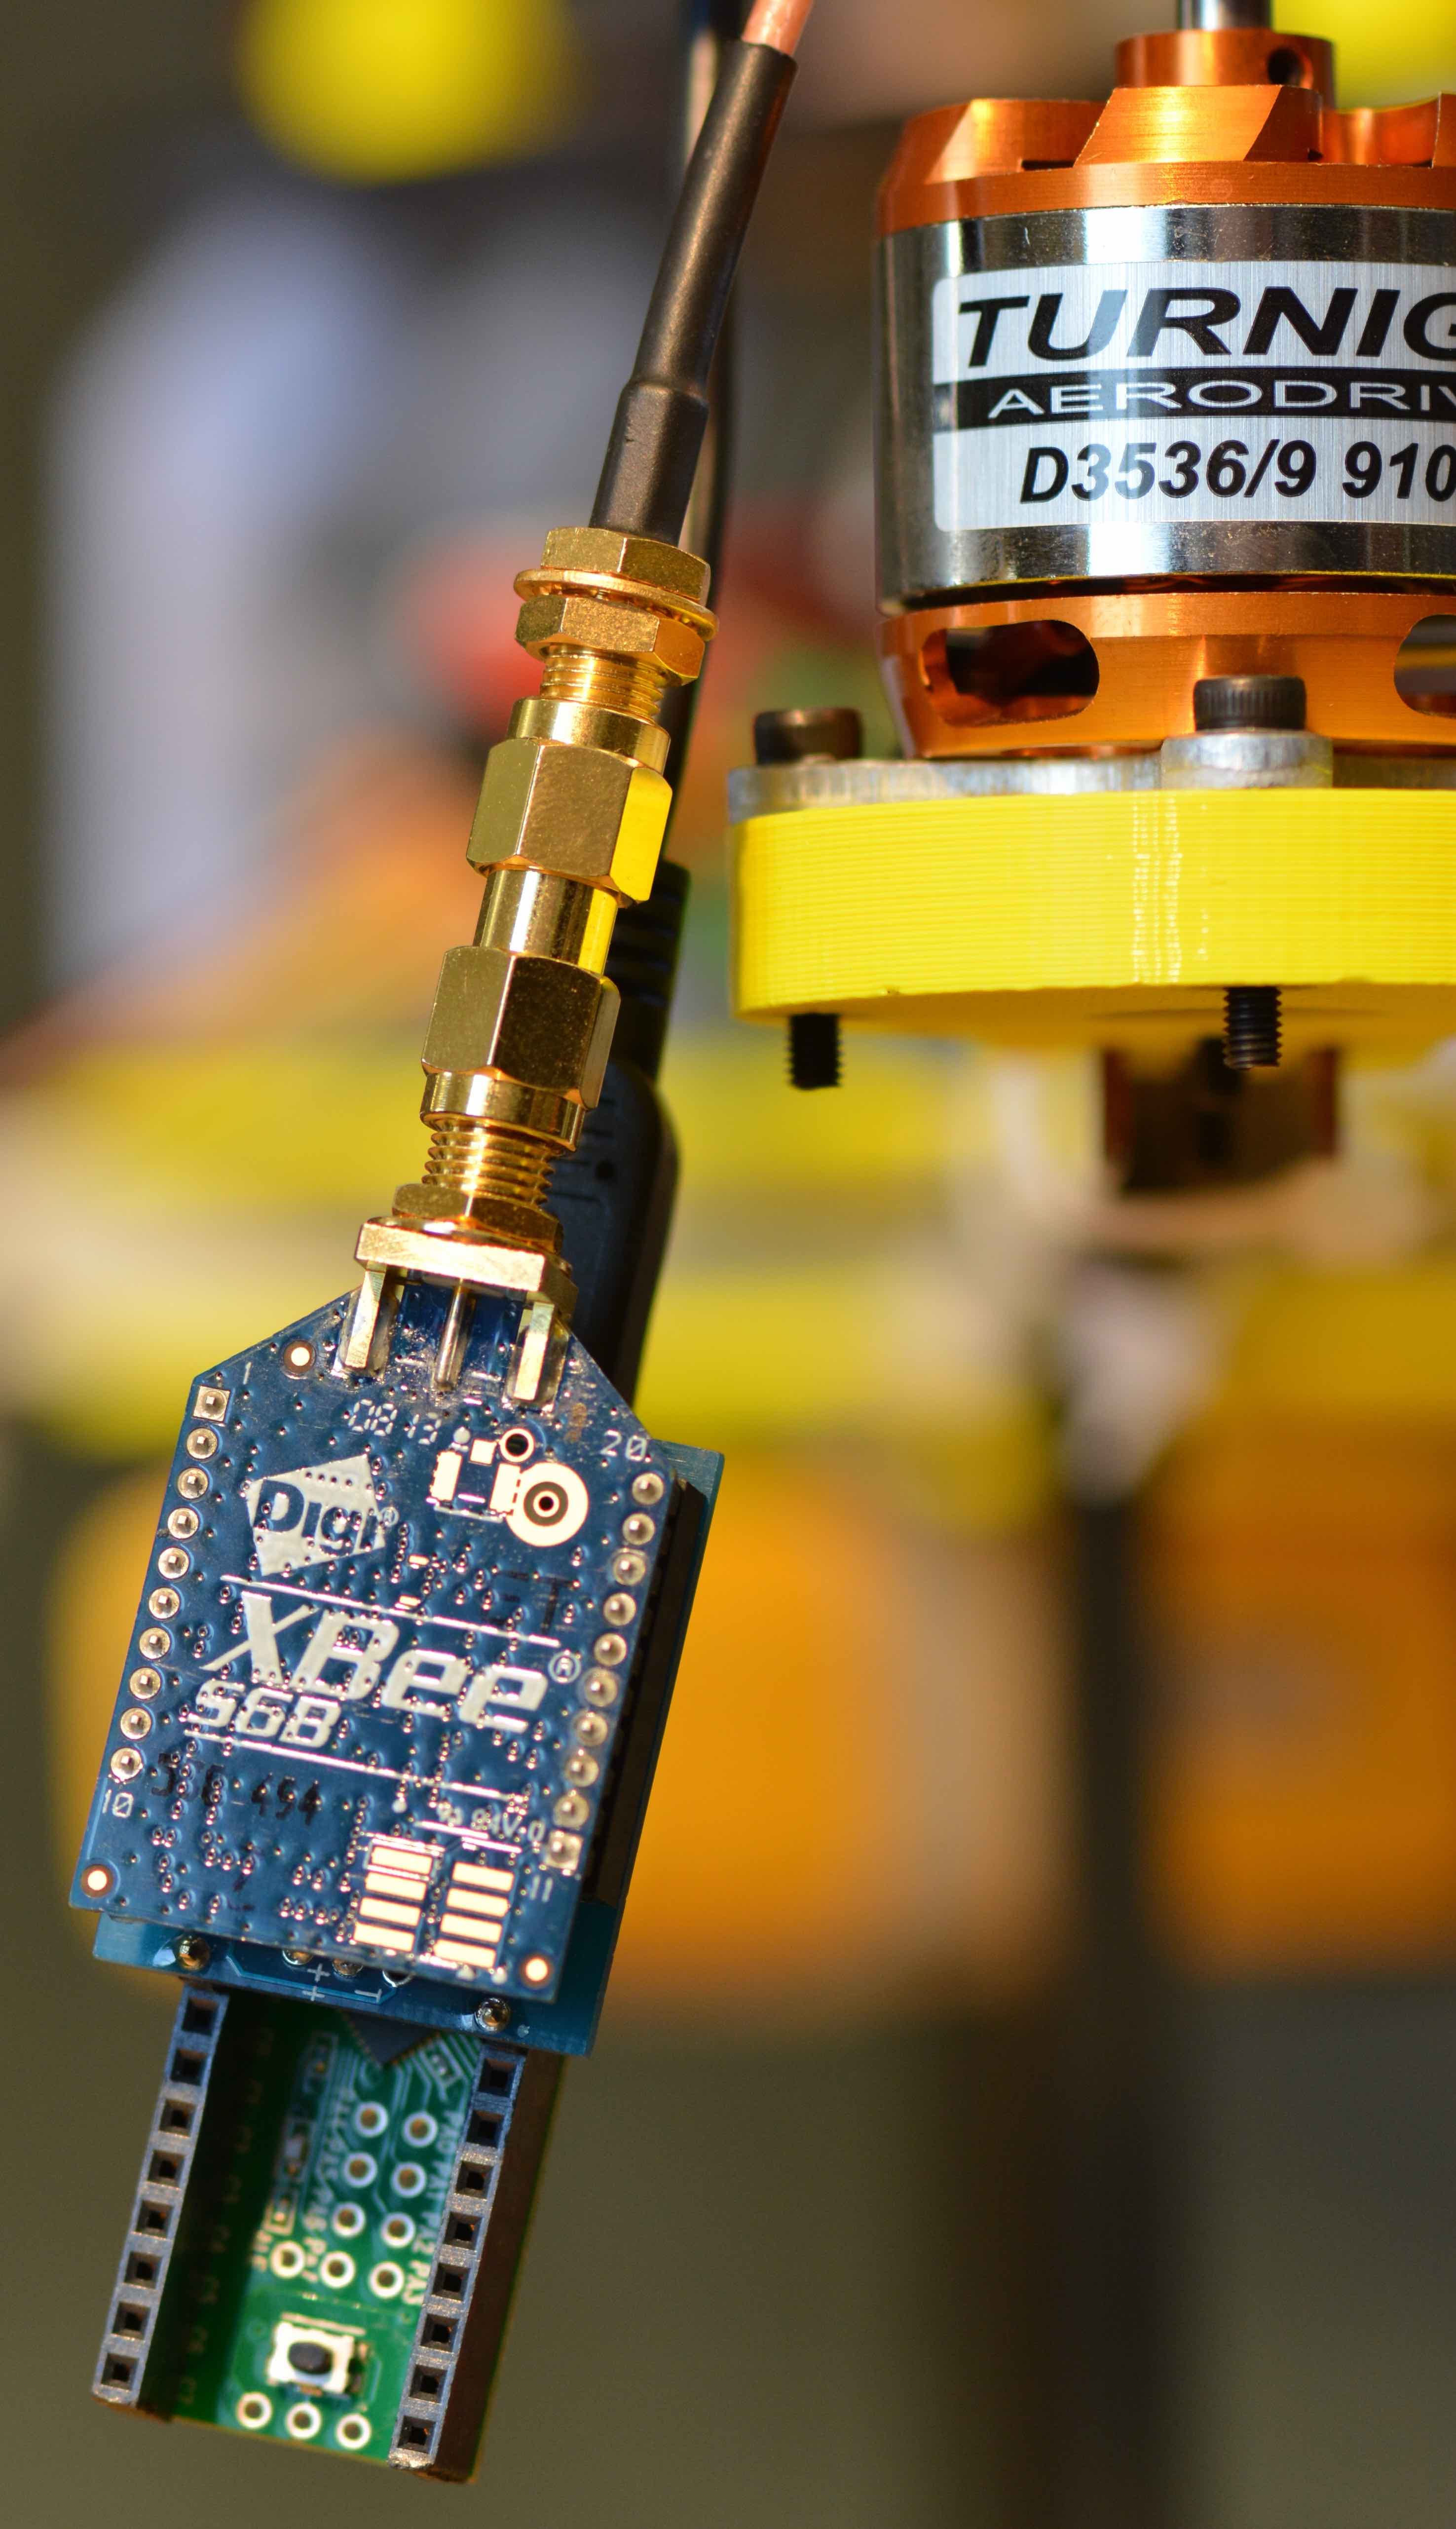
\includegraphics[width=1.2in]{Figures/Machine-Micro.jpg}
  \end{center}
\end{columns}
\end{frame}


\begin{frame}
\frametitle{Emerging Machine-Driven Traffic Characteristics}
\begin{center}
Anticipated traffic characteristics \textbf{invalidate acquisition-estimation-scheduling} paradigm!
\end{center}
\begin{columns}
\column{.45\textwidth}
  \begin{center}
  \scalebox{0.4}{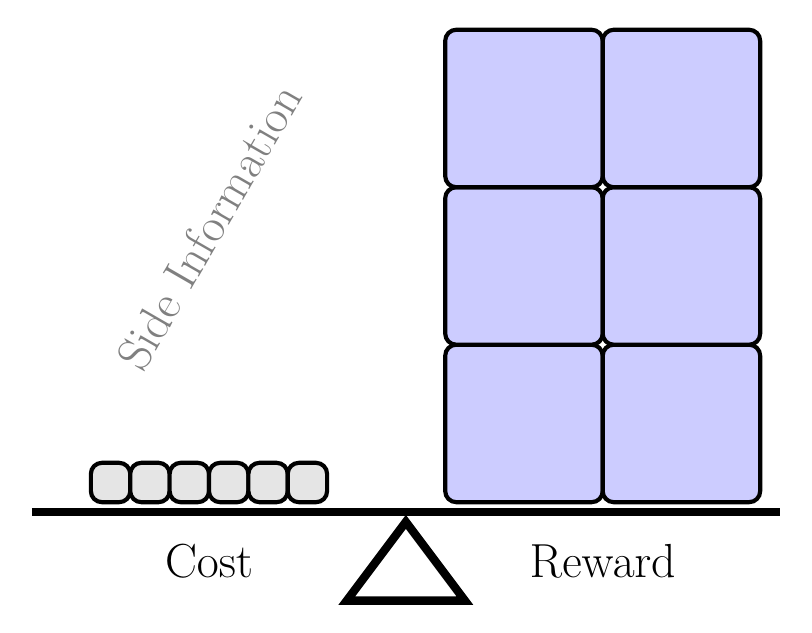
\begin{tikzpicture}
[draw=black, line width=1.5pt, >=stealth',
entry2/.style={rectangle, rounded corners, draw, fill=blue!20, inner sep=0pt, minimum size=20mm},
entry/.style={rectangle, rounded corners, draw, fill=gray!20, inner sep=0pt, minimum size=5mm}]

\node[entry] (r10) at (0.5,0) {};
\node[entry] (r20) at (1,0) {};
\node[entry] (r30) at (1.5,0) {};
\node[entry] (r40) at (2,0) {};
\node[entry] (r50) at (2.5,0) {};
\node[entry] (r60) at (3,0) {};

\node[entry2] (m00) at (5.75,0.75) {};
\node[entry2] (m01) at (5.75,2.75) {};
\node[entry2] (m02) at (5.75,4.75) {};
\node[entry2] (m00) at (7.75,0.75) {};
\node[entry2] (m11) at (7.75,2.75) {};
\node[entry2] (m12) at (7.75,4.75) {};

\draw[line width=3pt] (-0.5,-0.375) -- (9,-0.375);
\draw[line width=3pt] (3.5,-1.5) -- (4.25,-0.5) -- (5,-1.5) -- (3.5,-1.5) -- (4.25,-0.5);

\node (reward) at (1.75,-1) {\LARGE Cost};
\node (cost) at (6.75,-1) {\LARGE Reward};
\node[rotate=60] (info) at (1.75,3.25) {\LARGE \textcolor{gray}{Side Information}};
\end{tikzpicture}
}
  \end{center}
\column{.45\textwidth}
  \begin{center}
  \scalebox{0.4}{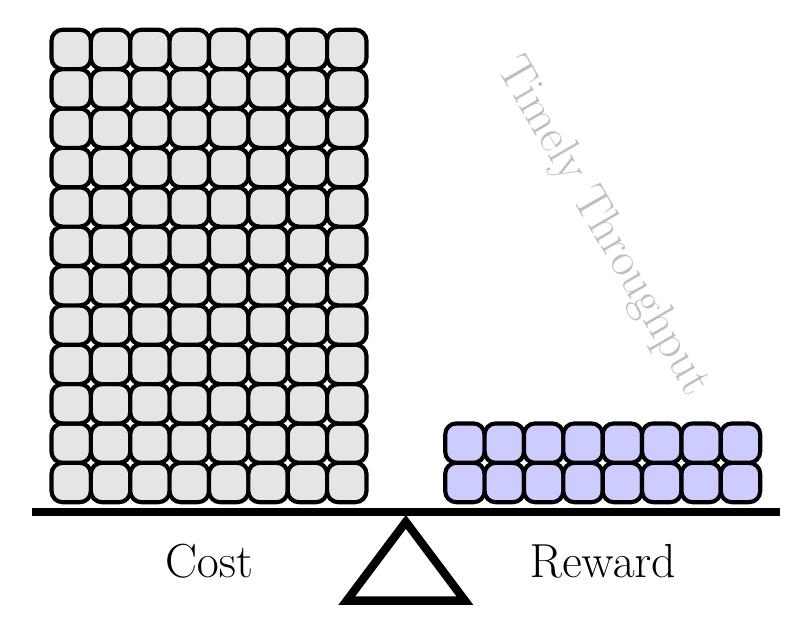
\begin{tikzpicture}
[draw=black, line width=1.5pt, >=stealth',
entry2/.style={rectangle, rounded corners, draw, fill=blue!20, inner sep=0pt, minimum size=5mm},
entry/.style={rectangle, rounded corners, draw, fill=gray!20, inner sep=0pt, minimum size=5mm}]

\node[entry] (m00) at (0,0) {};
\node[entry] (m01) at (0,0.5) {};
\node[entry] (m02) at (0,1) {};
\node[entry] (m03) at (0,1.5) {};
\node[entry] (m04) at (0,2) {};
\node[entry] (m05) at (0,2.5) {};
\node[entry] (m06) at (0,3) {};
\node[entry] (m07) at (0,3.5) {};
\node[entry] (m08) at (0,4) {};
\node[entry] (m09) at (0,4.5) {};
\node[entry] (m010) at (0,5) {};
\node[entry] (m011) at (0,5.5) {};

\node[entry] (m10) at (0.5,0) {};
\node[entry] (m11) at (0.5,0.5) {};
\node[entry] (m12) at (0.5,1) {};
\node[entry] (m13) at (0.5,1.5) {};
\node[entry] (m14) at (0.5,2) {};
\node[entry] (m15) at (0.5,2.5) {};
\node[entry] (m16) at (0.5,3) {};
\node[entry] (m17) at (0.5,3.5) {};
\node[entry] (m18) at (0.5,4) {};
\node[entry] (m19) at (0.5,4.5) {};
\node[entry] (m110) at (0.5,5) {};
\node[entry] (m111) at (0.5,5.5) {};

\node[entry] (m20) at (1,0) {};
\node[entry] (m21) at (1,0.5) {};
\node[entry] (m22) at (1,1) {};
\node[entry] (m23) at (1,1.5) {};
\node[entry] (m24) at (1,2) {};
\node[entry] (m25) at (1,2.5) {};
\node[entry] (m26) at (1,3) {};
\node[entry] (m27) at (1,3.5) {};
\node[entry] (m28) at (1,4) {};
\node[entry] (m29) at (1,4.5) {};
\node[entry] (m210) at (1,5) {};
\node[entry] (m211) at (1,5.5) {};

\node[entry] (m30) at (1.5,0) {};
\node[entry] (m31) at (1.5,0.5) {};
\node[entry] (m32) at (1.5,1) {};
\node[entry] (m33) at (1.5,1.5) {};
\node[entry] (m34) at (1.5,2) {};
\node[entry] (m35) at (1.5,2.5) {};
\node[entry] (m36) at (1.5,3) {};
\node[entry] (m37) at (1.5,3.5) {};
\node[entry] (m38) at (1.5,4) {};
\node[entry] (m39) at (1.5,4.5) {};
\node[entry] (m310) at (1.5,5) {};
\node[entry] (m311) at (1.5,5.5) {};

\node[entry] (m40) at (2,0) {};
\node[entry] (m41) at (2,0.5) {};
\node[entry] (m42) at (2,1) {};
\node[entry] (m43) at (2,1.5) {};
\node[entry] (m44) at (2,2) {};
\node[entry] (m45) at (2,2.5) {};
\node[entry] (m46) at (2,3) {};
\node[entry] (m47) at (2,3.5) {};
\node[entry] (m48) at (2,4) {};
\node[entry] (m49) at (2,4.5) {};
\node[entry] (m410) at (2,5) {};
\node[entry] (m411) at (2,5.5) {};

\node[entry] (m50) at (2.5,0) {};
\node[entry] (m51) at (2.5,0.5) {};
\node[entry] (m52) at (2.5,1) {};
\node[entry] (m53) at (2.5,1.5) {};
\node[entry] (m54) at (2.5,2) {};
\node[entry] (m55) at (2.5,2.5) {};
\node[entry] (m56) at (2.5,3) {};
\node[entry] (m57) at (2.5,3.5) {};
\node[entry] (m58) at (2.5,4) {};
\node[entry] (m59) at (2.5,4.5) {};
\node[entry] (m510) at (2.5,5) {};
\node[entry] (m511) at (2.5,5.5) {};

\node[entry] (m60) at (3,0) {};
\node[entry] (m61) at (3,0.5) {};
\node[entry] (m62) at (3,1) {};
\node[entry] (m63) at (3,1.5) {};
\node[entry] (m64) at (3,2) {};
\node[entry] (m65) at (3,2.5) {};
\node[entry] (m66) at (3,3) {};
\node[entry] (m67) at (3,3.5) {};
\node[entry] (m68) at (3,4) {};
\node[entry] (m69) at (3,4.5) {};
\node[entry] (m610) at (3,5) {};
\node[entry] (m611) at (3,5.5) {};

\node[entry] (m70) at (3.5,0) {};
\node[entry] (m71) at (3.5,0.5) {};
\node[entry] (m72) at (3.5,1) {};
\node[entry] (m73) at (3.5,1.5) {};
\node[entry] (m74) at (3.5,2) {};
\node[entry] (m75) at (3.5,2.5) {};
\node[entry] (m76) at (3.5,3) {};
\node[entry] (m77) at (3.5,3.5) {};
\node[entry] (m78) at (3.5,4) {};
\node[entry] (m79) at (3.5,4.5) {};
\node[entry] (m710) at (3.5,5) {};
\node[entry] (m711) at (3.5,5.5) {};

\node[entry2] (r00) at (5,0) {};
\node[entry2] (r01) at (5,0.5) {};

\node[entry2] (r10) at (5.5,0) {};
\node[entry2] (r11) at (5.5,0.5) {};

\node[entry2] (r20) at (6,0) {};
\node[entry2] (r21) at (6,0.5) {};

\node[entry2] (r30) at (6.5,0) {};
\node[entry2] (r31) at (6.5,0.5) {};

\node[entry2] (r40) at (7,0) {};
\node[entry2] (r41) at (7,0.5) {};

\node[entry2] (r50) at (7.5,0) {};
\node[entry2] (r51) at (7.5,0.5) {};

\node[entry2] (r60) at (8,0) {};
\node[entry2] (r61) at (8,0.5) {};

\node[entry2] (r70) at (8.5,0) {};
\node[entry2] (r71) at (8.5,0.5) {};

\draw[line width=3pt] (-0.5,-0.375) -- (9,-0.375);
\draw[line width=3pt] (3.5,-1.5) -- (4.25,-0.5) -- (5,-1.5) -- (3.5,-1.5) -- (4.25,-0.5);

\node (reward) at (1.75,-1) {\LARGE Cost};
\node (cost) at (6.75,-1) {\LARGE Reward};
\node[rotate=-60] (info) at (6.75,3.25) {\LARGE \textcolor{lightgray}{Timely Throughput}};
\end{tikzpicture}
}
  \end{center}
\end{columns}
\begin{block}{New Reality}
  \begin{itemize}
  \item Must address \textbf{sporadic} nature of machine-driven communications
  \item Transfer of \textbf{small payloads} without ability to amortize cost of acquiring channel and buffer states over long connections
  \item Preclude use of opportunistic scheduling
  \end{itemize}
\end{block}
\end{frame}


\begin{frame}
\frametitle{Uncoordinated and Unsourced MAC}
\begin{center}
\scalebox{0.75}{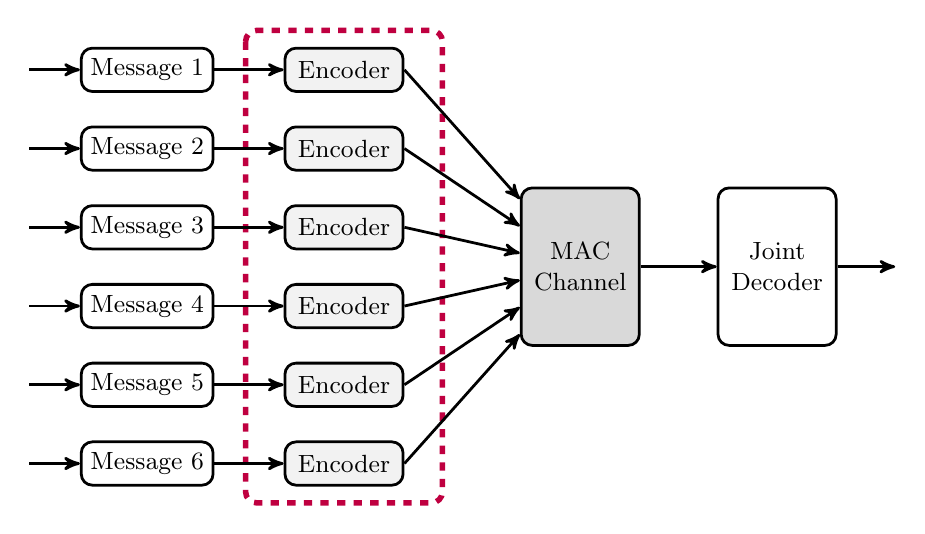
\begin{tikzpicture}
  [
  font=\small, draw=black, >=stealth', line width=1pt,
  channel/.style={rectangle, minimum height=20mm, minimum width=15mm, draw=black, fill=gray!30, rounded corners},
  encoder/.style={rectangle, minimum height=5.5mm, minimum width=15mm, draw=black, fill=gray!10, rounded corners},
  decoder/.style={rectangle, minimum height=20mm, minimum width=15mm, draw=black, rounded corners},
  message/.style={rectangle, minimum height=5.5mm, minimum width=15mm, draw=black, rounded corners}
  ]

\foreach \e in {1,2,3,4,5,6} {
  \node[encoder] (e\e) at (2.5,0.5-\e) {Encoder};
}

\draw[draw=purple, dashed, line width=2.0pt,rounded corners] (1.25, 0) rectangle (3.75, -6);

\foreach \m in {1,2,3,4,5,6} {
  \node[message] (m\m) at (0.0,0.5-\m) {Message~${\m}$}
  edge[->] (e\m);
  \draw[<-] (m\m) -- (-1.5,0.5-\m);
}
  
\node[channel,align=center] (channel) at (5.5,-3) {MAC\\Channel};
\node[decoder,align=center] (decoder) at (8,-3) {Joint\\Decoder};
\draw[->] (channel) -- (decoder);

\draw[->] (decoder.east) -- (9.5,-3);

\draw[->] (e1.east) -- (channel);
\draw[->] (e2.east) -- (channel);
\draw[->] (e3.east) -- (channel);
\draw[->] (e4.east) -- (channel);
\draw[->] (e5.east) -- (channel);
\draw[->] (e6.east) -- (channel);

\end{tikzpicture}
}
\end{center}
\begin{columns}
\column{.53\textwidth}
\begin{block}{Without Personalized Feedback}
  \begin{itemize}
  \item All devices employ same encoder
  \item No explicit knowledge of identities
  \item Need only return unordered list
  \end{itemize}
\end{block}
\column{.45\textwidth}
\begin{block}{Model}
  \begin{equation*}
  \textstyle \mathbf{y}
  = \sum_{i \in \mathbf{S}_{\mathrm{a}}} \mathbf{A} \mathbf{s}_i + \mathbf{n}
  \end{equation*}
  where $\mathbf{s}_i = f(\mathbf{w}_i)$ is codeword, only depends on message
\end{block}
\end{columns}
\myfootnote{\tiny
Y. Polyanskiy. \emph{A Perspective on Massive Random-Access}. ISIT, 2017}
\end{frame}


\begin{frame}
\frametitle{UMAC -- Compressed Sensing Interpretation}
\centerline{\centerline{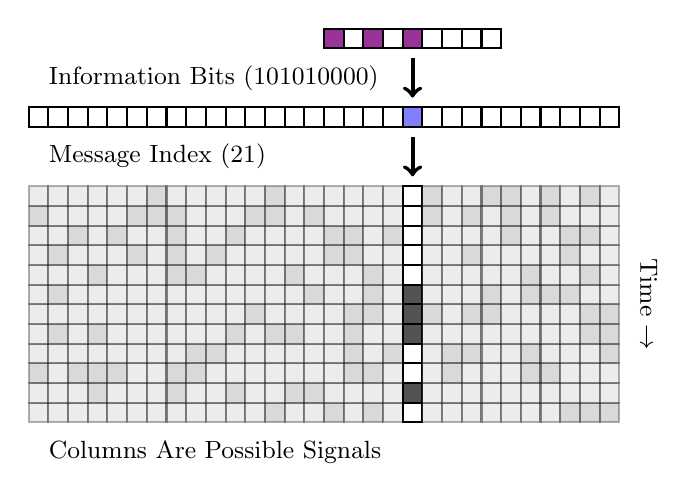
\begin{tikzpicture}
[font=\small, draw=black, line width=0.75pt,
bit0/.style={rectangle, draw, inner sep=0pt, minimum size=2.5mm},
bit1/.style={rectangle, draw, fill=violet!80, inner sep=0pt, minimum size=2.5mm},
entry0/.style={rectangle, draw, opacity=0.3, fill=lightgray, inner sep=0pt, minimum size=2.5mm},
entry1/.style={rectangle, draw, opacity=0.3, fill=gray, inner sep=0pt, minimum size=2.5mm},
entry00/.style={rectangle, draw, fill=white, inner sep=0pt, minimum size=2.5mm},
entry11/.style={rectangle, draw, fill=darkgray!90, inner sep=0pt, minimum size=2.5mm},
symbol0/.style={rectangle, draw, fill=white, inner sep=0pt, minimum size=2.5mm},
symbol1/.style={rectangle, draw, fill=blue!50, inner sep=0pt, minimum size=2.5mm}]

\node[entry0] (m0000) at (0.00,0) {};
\node[entry0] (m0100) at (0.25,0) {};
\node[entry0] (m0200) at (0.50,0) {};
\node[entry0] (m0300) at (0.75,0) {};
\node[entry0] (m0400) at (1.00,0) {};
\node[entry0] (m0500) at (1.25,0) {};
\node[entry0] (m0600) at (1.50,0) {};
\node[entry0] (m0700) at (1.75,0) {};
\node[entry0] (m0800) at (2.00,0) {};
\node[entry0] (m0900) at (2.25,0) {};
\node[entry0] (m1000) at (2.50,0) {};
\node[entry0] (m1100) at (2.75,0) {};
\node[entry1] (m1200) at (3.00,0) {};
\node[entry0] (m1300) at (3.25,0) {};
\node[entry0] (m1400) at (3.50,0) {};
\node[entry1] (m1500) at (3.75,0) {};
\node[entry0] (m1600) at (4.00,0) {};
\node[entry1] (m1700) at (4.25,0) {};
\node[entry0] (m1800) at (4.50,0) {};
\node[entry00] (m1900) at (4.75,0) {};
\node[entry0] (m2000) at (5.00,0) {};
\node[entry0] (m2100) at (5.25,0) {};
\node[entry0] (m2200) at (5.50,0) {};
\node[entry0] (m2300) at (5.75,0) {};
\node[entry0] (m2400) at (6.00,0) {};
\node[entry0] (m2500) at (6.25,0) {};
\node[entry0] (m2600) at (6.50,0) {};
\node[entry1] (m2700) at (6.75,0) {};
\node[entry1] (m2800) at (7.00,0) {};
\node[entry1] (m2900) at (7.25,0) {};

\node[entry0] (m0001) at (0.00,0.25) {};
\node[entry0] (m0101) at (0.25,0.25) {};
\node[entry0] (m0201) at (0.50,0.25) {};
\node[entry1] (m0301) at (0.75,0.25) {};
\node[entry0] (m0401) at (1.00,0.25) {};
\node[entry0] (m0501) at (1.25,0.25) {};
\node[entry0] (m0601) at (1.50,0.25) {};
\node[entry1] (m0701) at (1.75,0.25) {};
\node[entry0] (m0801) at (2.00,0.25) {};
\node[entry0] (m0901) at (2.25,0.25) {};
\node[entry1] (m1001) at (2.50,0.25) {};
\node[entry0] (m1101) at (2.75,0.25) {};
\node[entry0] (m1201) at (3.00,0.25) {};
\node[entry1] (m1301) at (3.25,0.25) {};
\node[entry1] (m1401) at (3.50,0.25) {};
\node[entry0] (m1501) at (3.75,0.25) {};
\node[entry0] (m1601) at (4.00,0.25) {};
\node[entry0] (m1701) at (4.25,0.25) {};
\node[entry0] (m1801) at (4.50,0.25) {};
\node[entry11] (m1901) at (4.75,0.25) {};
\node[entry0] (m2001) at (5.00,0.25) {};
\node[entry0] (m2101) at (5.25,0.25) {};
\node[entry0] (m2201) at (5.50,0.25) {};
\node[entry0] (m2301) at (5.75,0.25) {};
\node[entry0] (m2401) at (6.00,0.25) {};
\node[entry0] (m2501) at (6.25,0.25) {};
\node[entry0] (m2601) at (6.50,0.25) {};
\node[entry0] (m2701) at (6.75,0.25) {};
\node[entry0] (m2801) at (7.00,0.25) {};
\node[entry0] (m2901) at (7.25,0.25) {};

\node[entry1] (m0002) at (0.00,0.50) {};
\node[entry0] (m0102) at (0.25,0.50) {};
\node[entry1] (m0202) at (0.50,0.50) {};
\node[entry1] (m0302) at (0.75,0.50) {};
\node[entry1] (m0402) at (1.00,0.50) {};
\node[entry0] (m0502) at (1.25,0.50) {};
\node[entry0] (m0602) at (1.50,0.50) {};
\node[entry1] (m0702) at (1.75,0.50) {};
\node[entry1] (m0802) at (2.00,0.50) {};
\node[entry0] (m0902) at (2.25,0.50) {};
\node[entry0] (m1002) at (2.50,0.50) {};
\node[entry0] (m1102) at (2.75,0.50) {};
\node[entry0] (m1202) at (3.00,0.50) {};
\node[entry0] (m1302) at (3.25,0.50) {};
\node[entry0] (m1402) at (3.50,0.50) {};
\node[entry0] (m1502) at (3.75,0.50) {};
\node[entry1] (m1602) at (4.00,0.50) {};
\node[entry1] (m1702) at (4.25,0.50) {};
\node[entry0] (m1802) at (4.50,0.50) {};
\node[entry00] (m1902) at (4.75,0.50) {};
\node[entry0] (m2002) at (5.00,0.50) {};
\node[entry1] (m2102) at (5.25,0.50) {};
\node[entry0] (m2202) at (5.50,0.50) {};
\node[entry0] (m2302) at (5.75,0.50) {};
\node[entry0] (m2402) at (6.00,0.50) {};
\node[entry1] (m2502) at (6.25,0.50) {};
\node[entry1] (m2602) at (6.50,0.50) {};
\node[entry0] (m2702) at (6.75,0.50) {};
\node[entry0] (m2802) at (7.00,0.50) {};
\node[entry0] (m2902) at (7.25,0.50) {};

\node[entry0] (m0003) at (0.00,0.75) {};
\node[entry0] (m0103) at (0.25,0.75) {};
\node[entry0] (m0203) at (0.50,0.75) {};
\node[entry0] (m0303) at (0.75,0.75) {};
\node[entry0] (m0403) at (1.00,0.75) {};
\node[entry0] (m0503) at (1.25,0.75) {};
\node[entry0] (m0603) at (1.50,0.75) {};
\node[entry0] (m0703) at (1.75,0.75) {};
\node[entry1] (m0803) at (2.00,0.75) {};
\node[entry1] (m0903) at (2.25,0.75) {};
\node[entry0] (m1003) at (2.50,0.75) {};
\node[entry0] (m1103) at (2.75,0.75) {};
\node[entry0] (m1203) at (3.00,0.75) {};
\node[entry0] (m1303) at (3.25,0.75) {};
\node[entry0] (m1403) at (3.50,0.75) {};
\node[entry0] (m1503) at (3.75,0.75) {};
\node[entry1] (m1603) at (4.00,0.75) {};
\node[entry0] (m1703) at (4.25,0.75) {};
\node[entry1] (m1803) at (4.50,0.75) {};
\node[entry00] (m1903) at (4.75,0.75) {};
\node[entry0] (m2003) at (5.00,0.75) {};
\node[entry1] (m2103) at (5.25,0.75) {};
\node[entry1] (m2203) at (5.50,0.75) {};
\node[entry0] (m2303) at (5.75,0.75) {};
\node[entry0] (m2403) at (6.00,0.75) {};
\node[entry1] (m2503) at (6.25,0.75) {};
\node[entry0] (m2603) at (6.50,0.75) {};
\node[entry0] (m2703) at (6.75,0.75) {};
\node[entry0] (m2803) at (7.00,0.75) {};
\node[entry1] (m2903) at (7.25,0.75) {};

\node[entry0] (m0004) at (0.00,1.00) {};
\node[entry1] (m0104) at (0.25,1.00) {};
\node[entry0] (m0204) at (0.50,1.00) {};
\node[entry1] (m0304) at (0.75,1.00) {};
\node[entry0] (m0404) at (1.00,1.00) {};
\node[entry0] (m0504) at (1.25,1.00) {};
\node[entry0] (m0604) at (1.50,1.00) {};
\node[entry0] (m0704) at (1.75,1.00) {};
\node[entry0] (m0804) at (2.00,1.00) {};
\node[entry0] (m0904) at (2.25,1.00) {};
\node[entry1] (m1004) at (2.50,1.00) {};
\node[entry0] (m1104) at (2.75,1.00) {};
\node[entry1] (m1204) at (3.00,1.00) {};
\node[entry1] (m1304) at (3.25,1.00) {};
\node[entry0] (m1404) at (3.50,1.00) {};
\node[entry0] (m1504) at (3.75,1.00) {};
\node[entry1] (m1604) at (4.00,1.00) {};
\node[entry0] (m1704) at (4.25,1.00) {};
\node[entry0] (m1804) at (4.50,1.00) {};
\node[entry11] (m1904) at (4.75,1.00) {};
\node[entry0] (m2004) at (5.00,1.00) {};
\node[entry0] (m2104) at (5.25,1.00) {};
\node[entry0] (m2204) at (5.50,1.00) {};
\node[entry0] (m2304) at (5.75,1.00) {};
\node[entry0] (m2404) at (6.00,1.00) {};
\node[entry0] (m2504) at (6.25,1.00) {};
\node[entry0] (m2604) at (6.50,1.00) {};
\node[entry0] (m2704) at (6.75,1.00) {};
\node[entry1] (m2804) at (7.00,1.00) {};
\node[entry1] (m2904) at (7.25,1.00) {};

\node[entry0] (m0005) at (0.00,1.25) {};
\node[entry0] (m0105) at (0.25,1.25) {};
\node[entry0] (m0205) at (0.50,1.25) {};
\node[entry0] (m0305) at (0.75,1.25) {};
\node[entry0] (m0405) at (1.00,1.25) {};
\node[entry0] (m0505) at (1.25,1.25) {};
\node[entry0] (m0605) at (1.50,1.25) {};
\node[entry0] (m0705) at (1.75,1.25) {};
\node[entry0] (m0805) at (2.00,1.25) {};
\node[entry0] (m0905) at (2.25,1.25) {};
\node[entry0] (m1005) at (2.50,1.25) {};
\node[entry1] (m1105) at (2.75,1.25) {};
\node[entry0] (m1205) at (3.00,1.25) {};
\node[entry0] (m1305) at (3.25,1.25) {};
\node[entry0] (m1405) at (3.50,1.25) {};
\node[entry0] (m1505) at (3.75,1.25) {};
\node[entry1] (m1605) at (4.00,1.25) {};
\node[entry1] (m1705) at (4.25,1.25) {};
\node[entry0] (m1805) at (4.50,1.25) {};
\node[entry11] (m1905) at (4.75,1.25) {};
\node[entry1] (m2005) at (5.00,1.25) {};
\node[entry0] (m2105) at (5.25,1.25) {};
\node[entry1] (m2205) at (5.50,1.25) {};
\node[entry1] (m2305) at (5.75,1.25) {};
\node[entry0] (m2405) at (6.00,1.25) {};
\node[entry0] (m2505) at (6.25,1.25) {};
\node[entry0] (m2605) at (6.50,1.25) {};
\node[entry0] (m2705) at (6.75,1.25) {};
\node[entry1] (m2805) at (7.00,1.25) {};
\node[entry1] (m2905) at (7.25,1.25) {};

\node[entry0] (m0006) at (0.00,1.50) {};
\node[entry1] (m0106) at (0.25,1.50) {};
\node[entry0] (m0206) at (0.50,1.50) {};
\node[entry0] (m0306) at (0.75,1.50) {};
\node[entry0] (m0406) at (1.00,1.50) {};
\node[entry0] (m0506) at (1.25,1.50) {};
\node[entry0] (m0606) at (1.50,1.50) {};
\node[entry0] (m0706) at (1.75,1.50) {};
\node[entry0] (m0806) at (2.00,1.50) {};
\node[entry0] (m0906) at (2.25,1.50) {};
\node[entry0] (m1006) at (2.50,1.50) {};
\node[entry0] (m1106) at (2.75,1.50) {};
\node[entry0] (m1206) at (3.00,1.50) {};
\node[entry0] (m1306) at (3.25,1.50) {};
\node[entry1] (m1406) at (3.50,1.50) {};
\node[entry0] (m1506) at (3.75,1.50) {};
\node[entry0] (m1606) at (4.00,1.50) {};
\node[entry1] (m1706) at (4.25,1.50) {};
\node[entry0] (m1806) at (4.50,1.50) {};
\node[entry11] (m1906) at (4.75,1.50) {};
\node[entry0] (m2006) at (5.00,1.50) {};
\node[entry0] (m2106) at (5.25,1.50) {};
\node[entry0] (m2206) at (5.50,1.50) {};
\node[entry1] (m2306) at (5.75,1.50) {};
\node[entry0] (m2406) at (6.00,1.50) {};
\node[entry1] (m2506) at (6.25,1.50) {};
\node[entry1] (m2606) at (6.50,1.50) {};
\node[entry1] (m2706) at (6.75,1.50) {};
\node[entry0] (m2806) at (7.00,1.50) {};
\node[entry0] (m2906) at (7.25,1.50) {};

\node[entry0] (m0007) at (0.00,1.75) {};
\node[entry0] (m0107) at (0.25,1.75) {};
\node[entry0] (m0207) at (0.50,1.75) {};
\node[entry1] (m0307) at (0.75,1.75) {};
\node[entry0] (m0407) at (1.00,1.75) {};
\node[entry0] (m0507) at (1.25,1.75) {};
\node[entry0] (m0607) at (1.50,1.75) {};
\node[entry1] (m0707) at (1.75,1.75) {};
\node[entry1] (m0807) at (2.00,1.75) {};
\node[entry0] (m0907) at (2.25,1.75) {};
\node[entry0] (m1007) at (2.50,1.75) {};
\node[entry0] (m1107) at (2.75,1.75) {};
\node[entry0] (m1207) at (3.00,1.75) {};
\node[entry1] (m1307) at (3.25,1.75) {};
\node[entry0] (m1407) at (3.50,1.75) {};
\node[entry0] (m1507) at (3.75,1.75) {};
\node[entry0] (m1607) at (4.00,1.75) {};
\node[entry1] (m1707) at (4.25,1.75) {};
\node[entry0] (m1807) at (4.50,1.75) {};
\node[entry00] (m1907) at (4.75,1.75) {};
\node[entry0] (m2007) at (5.00,1.75) {};
\node[entry0] (m2107) at (5.25,1.75) {};
\node[entry0] (m2207) at (5.50,1.75) {};
\node[entry0] (m2307) at (5.75,1.75) {};
\node[entry0] (m2407) at (6.00,1.75) {};
\node[entry1] (m2507) at (6.25,1.75) {};
\node[entry0] (m2607) at (6.50,1.75) {};
\node[entry0] (m2707) at (6.75,1.75) {};
\node[entry1] (m2807) at (7.00,1.75) {};
\node[entry0] (m2907) at (7.25,1.75) {};

\node[entry0] (m0008) at (0.00,2.00) {};
\node[entry1] (m0108) at (0.25,2.00) {};
\node[entry0] (m0208) at (0.50,2.00) {};
\node[entry0] (m0308) at (0.75,2.00) {};
\node[entry0] (m0408) at (1.00,2.00) {};
\node[entry1] (m0508) at (1.25,2.00) {};
\node[entry0] (m0608) at (1.50,2.00) {};
\node[entry1] (m0708) at (1.75,2.00) {};
\node[entry0] (m0808) at (2.00,2.00) {};
\node[entry1] (m0908) at (2.25,2.00) {};
\node[entry0] (m1008) at (2.50,2.00) {};
\node[entry0] (m1108) at (2.75,2.00) {};
\node[entry0] (m1208) at (3.00,2.00) {};
\node[entry0] (m1308) at (3.25,2.00) {};
\node[entry0] (m1408) at (3.50,2.00) {};
\node[entry1] (m1508) at (3.75,2.00) {};
\node[entry1] (m1608) at (4.00,2.00) {};
\node[entry0] (m1708) at (4.25,2.00) {};
\node[entry0] (m1808) at (4.50,2.00) {};
\node[entry00] (m1908) at (4.75,2.00) {};
\node[entry0] (m2008) at (5.00,2.00) {};
\node[entry0] (m2108) at (5.25,2.00) {};
\node[entry1] (m2208) at (5.50,2.00) {};
\node[entry0] (m2308) at (5.75,2.00) {};
\node[entry0] (m2408) at (6.00,2.00) {};
\node[entry0] (m2508) at (6.25,2.00) {};
\node[entry0] (m2608) at (6.50,2.00) {};
\node[entry1] (m2708) at (6.75,2.00) {};
\node[entry0] (m2808) at (7.00,2.00) {};
\node[entry0] (m2908) at (7.25,2.00) {};

\node[entry0] (m0009) at (0.00,2.25) {};
\node[entry0] (m0109) at (0.25,2.25) {};
\node[entry1] (m0209) at (0.50,2.25) {};
\node[entry0] (m0309) at (0.75,2.25) {};
\node[entry1] (m0409) at (1.00,2.25) {};
\node[entry0] (m0509) at (1.25,2.25) {};
\node[entry0] (m0609) at (1.50,2.25) {};
\node[entry1] (m0709) at (1.75,2.25) {};
\node[entry0] (m0809) at (2.00,2.25) {};
\node[entry0] (m0909) at (2.25,2.25) {};
\node[entry1] (m1009) at (2.50,2.25) {};
\node[entry0] (m1109) at (2.75,2.25) {};
\node[entry0] (m1209) at (3.00,2.25) {};
\node[entry0] (m1309) at (3.25,2.25) {};
\node[entry0] (m1409) at (3.50,2.25) {};
\node[entry1] (m1509) at (3.75,2.25) {};
\node[entry1] (m1609) at (4.00,2.25) {};
\node[entry0] (m1709) at (4.25,2.25) {};
\node[entry1] (m1809) at (4.50,2.25) {};
\node[entry00] (m1909) at (4.75,2.25) {};
\node[entry0] (m2009) at (5.00,2.25) {};
\node[entry0] (m2109) at (5.25,2.25) {};
\node[entry0] (m2209) at (5.50,2.25) {};
\node[entry0] (m2309) at (5.75,2.25) {};
\node[entry1] (m2409) at (6.00,2.25) {};
\node[entry0] (m2509) at (6.25,2.25) {};
\node[entry0] (m2609) at (6.50,2.25) {};
\node[entry1] (m2709) at (6.75,2.25) {};
\node[entry1] (m2809) at (7.00,2.25) {};
\node[entry0] (m2909) at (7.25,2.25) {};

\node[entry1] (m0010) at (0.00,2.50) {};
\node[entry0] (m0110) at (0.25,2.50) {};
\node[entry0] (m0210) at (0.50,2.50) {};
\node[entry0] (m0310) at (0.75,2.50) {};
\node[entry0] (m0410) at (1.00,2.50) {};
\node[entry1] (m0510) at (1.25,2.50) {};
\node[entry1] (m0610) at (1.50,2.50) {};
\node[entry1] (m0710) at (1.75,2.50) {};
\node[entry0] (m0810) at (2.00,2.50) {};
\node[entry0] (m0910) at (2.25,2.50) {};
\node[entry0] (m1010) at (2.50,2.50) {};
\node[entry1] (m1110) at (2.75,2.50) {};
\node[entry1] (m1210) at (3.00,2.50) {};
\node[entry0] (m1310) at (3.25,2.50) {};
\node[entry1] (m1410) at (3.50,2.50) {};
\node[entry0] (m1510) at (3.75,2.50) {};
\node[entry0] (m1610) at (4.00,2.50) {};
\node[entry0] (m1710) at (4.25,2.50) {};
\node[entry0] (m1810) at (4.50,2.50) {};
\node[entry00] (m1910) at (4.75,2.50) {};
\node[entry1] (m2010) at (5.00,2.50) {};
\node[entry0] (m2110) at (5.25,2.50) {};
\node[entry1] (m2210) at (5.50,2.50) {};
\node[entry0] (m2310) at (5.75,2.50) {};
\node[entry1] (m2410) at (6.00,2.50) {};
\node[entry0] (m2510) at (6.25,2.50) {};
\node[entry1] (m2610) at (6.50,2.50) {};
\node[entry0] (m2710) at (6.75,2.50) {};
\node[entry0] (m2810) at (7.00,2.50) {};
\node[entry0] (m2910) at (7.25,2.50) {};

\node[entry0] (m0011) at (0.00,2.75) {};
\node[entry0] (m0111) at (0.25,2.75) {};
\node[entry0] (m0211) at (0.50,2.75) {};
\node[entry0] (m0311) at (0.75,2.75) {};
\node[entry0] (m0411) at (1.00,2.75) {};
\node[entry0] (m0511) at (1.25,2.75) {};
\node[entry1] (m0611) at (1.50,2.75) {};
\node[entry0] (m0711) at (1.75,2.75) {};
\node[entry0] (m0811) at (2.00,2.75) {};
\node[entry0] (m0911) at (2.25,2.75) {};
\node[entry0] (m1011) at (2.50,2.75) {};
\node[entry0] (m1111) at (2.75,2.75) {};
\node[entry1] (m1211) at (3.00,2.75) {};
\node[entry0] (m1311) at (3.25,2.75) {};
\node[entry0] (m1411) at (3.50,2.75) {};
\node[entry0] (m1511) at (3.75,2.75) {};
\node[entry0] (m1611) at (4.00,2.75) {};
\node[entry0] (m1711) at (4.25,2.75) {};
\node[entry0] (m1811) at (4.50,2.75) {};
\node[entry00] (m1911) at (4.75,2.75) {};
\node[entry1] (m2011) at (5.00,2.75) {};
\node[entry0] (m2111) at (5.25,2.75) {};
\node[entry0] (m2211) at (5.50,2.75) {};
\node[entry1] (m2311) at (5.75,2.75) {};
\node[entry1] (m2411) at (6.00,2.75) {};
\node[entry0] (m2511) at (6.25,2.75) {};
\node[entry1] (m2611) at (6.50,2.75) {};
\node[entry0] (m2711) at (6.75,2.75) {};
\node[entry1] (m2811) at (7.00,2.75) {};
\node[entry0] (m2911) at (7.25,2.75) {};

\draw[->, line width=1.5pt]  (4.75,3.50) -- (4.75,3.00);

\node[symbol0] (s00) at (0.00,3.75) {};
\node[symbol0] (s01) at (0.25,3.75) {};
\node[symbol0] (s02) at (0.50,3.75) {};
\node[symbol0] (s03) at (0.75,3.75) {};
\node[symbol0] (s04) at (1.00,3.75) {};
\node[symbol0] (s05) at (1.25,3.75) {};
\node[symbol0] (s06) at (1.50,3.75) {};
\node[symbol0] (s07) at (1.75,3.75) {};
\node[symbol0] (s08) at (2.00,3.75) {};
\node[symbol0] (s09) at (2.25,3.75) {};
\node[symbol0] (s10) at (2.50,3.75) {};
\node[symbol0] (s11) at (2.75,3.75) {};
\node[symbol0] (s12) at (3.00,3.75) {};
\node[symbol0] (s13) at (3.25,3.75) {};
\node[symbol0] (s14) at (3.50,3.75) {};
\node[symbol0] (s15) at (3.75,3.75) {};
\node[symbol0] (s16) at (4.00,3.75) {};
\node[symbol0] (s17) at (4.25,3.75) {};
\node[symbol0] (s18) at (4.50,3.75) {};
\node[symbol1] (s19) at (4.75,3.75) {};
\node[symbol0] (s20) at (5.00,3.75) {};
\node[symbol0] (s21) at (5.25,3.75) {};
\node[symbol0] (s22) at (5.50,3.75) {};
\node[symbol0] (s23) at (5.75,3.75) {};
\node[symbol0] (s24) at (6.00,3.75) {};
\node[symbol0] (s25) at (6.25,3.75) {};
\node[symbol0] (s26) at (6.50,3.75) {};
\node[symbol0] (s27) at (6.75,3.75) {};
\node[symbol0] (s28) at (7.00,3.75) {};
\node[symbol0] (s29) at (7.25,3.75) {};

\draw[->, line width=1.5pt]  (4.75,4.50) -- (4.75,4.00);

\node[bit1] (info0) at (3.75,4.75) {};
\node[bit0] (info1) at (4.00,4.75) {};
\node[bit1] (info2) at (4.25,4.75) {};
\node[bit0] (info3) at (4.50,4.75) {};
\node[bit1] (info4) at (4.75,4.75) {};
\node[bit0] (info5) at (5.00,4.75) {};
\node[bit0] (info6) at (5.25,4.75) {};
\node[bit0] (info7) at (5.50,4.75) {};
\node[bit0] (info8) at (5.75,4.75) {};


\node [anchor = west] (infobits) at (0.00,4.25) {Information Bits (101010000)};
\node [anchor = west] (messageindex) at (0.00,3.25) {Message Index (21)};
\node [anchor = west] (signals) at (0.00,-0.50) {Columns Are Possible Signals};
\node[rotate=-90] (time) at (7.75,1.375) {Time $\rightarrow$};
\end{tikzpicture}
}}
\vfill
\begin{itemize}
\item Bit sequence $\mathbf{w}_i \in \{ 0,1 \}^B$ converted to index $\mathbf{s}_i$ in $[0,2^B-1]$
\item Stack codewords into $N \times 2^B$ \emph{sensing} matrix with $B \approx 128$
\item Message index determines transmitted codeword
\end{itemize}
\end{frame}


\begin{frame}
\frametitle{Quest for Low-Complexity Unsourced MAC}
\begin{block}{Idea~1: Divide and Conquer Information Bits}
\begin{center}
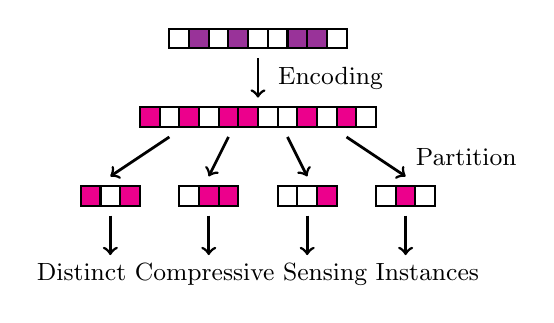
\begin{tikzpicture}
[font=\small, draw=black, line width=0.75pt,
bit0/.style={rectangle, draw, inner sep=0pt, minimum size=2.5mm},
bit1/.style={rectangle, draw, fill=violet!80, inner sep=0pt, minimum size=2.5mm},
ebit0/.style={rectangle, draw, inner sep=0pt, minimum size=2.5mm},
ebit1/.style={rectangle, draw, fill=magenta, inner sep=0pt, minimum size=2.5mm}
]

\node[bit0] (info0) at (0.875,5) {};
\node[bit1] (info1) at (1.125,5) {};
\node[bit0] (info2) at (1.375,5) {};
\node[bit1] (info3) at (1.625,5) {};
\node[bit0] (info4) at (1.875,5) {};
\node[bit0] (info5) at (2.125,5) {};
\node[bit1] (info6) at (2.375,5) {};
\node[bit1] (info7) at (2.625,5) {};
\node[bit0] (info8) at (2.875,5) {};

\draw[->, line width=1pt]  (1.875,4.75) -- (1.875,4.25);
\node[anchor=west] (coding) at (2,4.50) {Encoding};

\node[ebit1] (ebit0) at (0.50,4) {};
\node[ebit0] (ebit1) at (0.75,4) {};
\node[ebit1] (ebit2) at (1.00,4) {};
\node[ebit0] (ebit3) at (1.25,4) {};
\node[ebit1] (ebit4) at (1.50,4) {};
\node[ebit1] (ebit5) at (1.75,4) {};
\node[ebit0] (ebit6) at (2.00,4) {};
\node[ebit0] (ebit7) at (2.25,4) {};
\node[ebit1] (ebit8) at (2.50,4) {};
\node[ebit0] (ebit9) at (2.75,4) {};
\node[ebit1] (ebit10) at (3.00,4) {};
\node[ebit0] (ebit11) at (3.25,4) {};

\draw[->, line width=1pt]  (0.75,3.75) -- (0.00,3.25);
\draw[->, line width=1pt]  (1.50,3.75) -- (1.25,3.25);
\draw[->, line width=1pt]  (2.25,3.75) -- (2.50,3.25);
\draw[->, line width=1pt]  (3.00,3.75) -- (3.75,3.25);
\node[anchor=west] (coding) at (3.75,3.50) {Partition};

\node[ebit1] (s00) at (-0.25,3.00) {};
\node[ebit0] (s01) at (0.00,3.00) {};
\node[ebit1] (s02) at (0.25,3.00) {};

\node[ebit0] (s03) at (1.00,3.00) {};
\node[ebit1] (s04) at (1.25,3.00) {};
\node[ebit1] (s05) at (1.50,3.00) {};

\node[ebit0] (s06) at (2.25,3.00) {};
\node[ebit0] (s07) at (2.50,3.00) {};
\node[ebit1] (s08) at (2.75,3.00) {};

\node[ebit0] (s09) at (3.50,3.00) {};
\node[ebit1] (s10) at (3.75,3.00) {};
\node[ebit0] (s11) at (4.00,3.00) {};

\draw[->, line width=1pt]  (0.00,2.75) -- (0.00,2.25);
\draw[->, line width=1pt]  (1.25,2.75) -- (1.25,2.25);
\draw[->, line width=1pt]  (2.50,2.75) -- (2.50,2.25);
\draw[->, line width=1pt]  (3.75,2.75) -- (3.75,2.25);

\node (cs) at (1.875,2.00) {Distinct Compressive Sensing Instances};
\end{tikzpicture}

\end{center}
\begin{itemize}
\item Split problem into sub-components suitable for CS framework
\item Get lists of sub-packets, one list for every slot
\item Stitch pieces of one packet together using error correction
\end{itemize}
\end{block}
\end{frame}


\begin{frame}
\frametitle{Coded Compressive Sensing -- Device Perspective}
\centerline{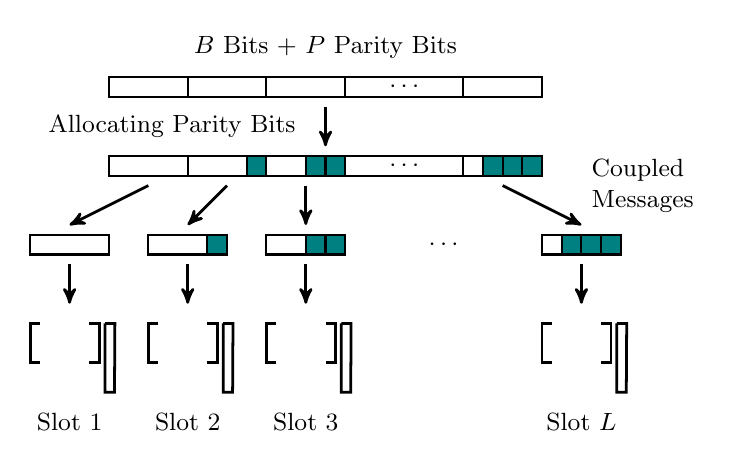
\begin{tikzpicture}
[font=\small, draw=black, line width=0.75pt, >=stealth',
sub0/.style={rectangle, draw, inner sep=0pt, minimum width=10mm,  minimum height=2.5mm},
sub1/.style={rectangle, draw, inner sep=0pt, minimum width=15mm, minimum height=2.5mm},
sub1s/.style={rectangle, inner sep=0pt, minimum width=15mm, minimum height=2.5mm},
parity/.style={rectangle, draw, fill=teal, inner sep=0pt, minimum size=2.5mm}]

\node (coupledvector) at (2.25,5.50) {$B$~Bits + $P$~Parity Bits};
\node[sub0] (cs0) at (0.00,5) {};
\node[sub0] (cs2) at (1.00,5) {};
\node[sub0] (cs3) at (2.00,5) {};
\node[sub1] (csx) at (3.25,5) {$\cdots$};
\node[sub0] (csz) at (4.50,5) {};

\draw[->, line width=1pt]  (2.25,4.75) -- (2.25,4.25);
\node[anchor=east] (coding) at (2.00,4.50) {Allocating Parity Bits};

\node[sub0] (subcs0) at (0.00,4) {};
\node[sub0] (subcs2) at (1.00,4) {};
\node[parity] (parity0) at (1.375,4) {};
\node[sub0] (subcs3) at (2.00,4) {};
\node[parity] (parity1) at (2.125,4) {};
\node[parity] (parity2) at (2.375,4) {};
\node[sub1] (subcsx) at (3.25,4) {$\cdots$};
\node[sub0] (subcsz) at (4.50,4) {};
\node[parity] (parity3) at (4.375,4) {};
\node[parity] (parity4) at (4.625,4) {};
\node[parity] (parity5) at (4.875,4) {};

\node[sub0] (subcs0) at (-1.00,3) {};
\node[sub0] (subcs2) at (0.50,3) {};
\node[parity] (parity0) at (0.875,3) {};
\node[sub0] (subcs3) at (2.00,3) {};
\node[parity] (parity1) at (2.125,3) {};
\node[parity] (parity2) at (2.375,3) {};
\node[sub1s] (subcsx) at (3.75,3) {$\cdots$};
\node[sub0] (subcsz) at (5.50,3) {};
\node[parity] (parity3) at (5.375,3) {};
\node[parity] (parity4) at (5.625,3) {};
\node[parity] (parity5) at (5.875,3) {};

\draw[->, line width=1pt]  (0.00,3.75) -- (-1.00,3.25);
\draw[->, line width=1pt]  (1.00,3.75) -- (0.50,3.25);
\draw[->, line width=1pt]  (2.00,3.75) -- (2.00,3.25);
\draw[->, line width=1pt]  (4.50,3.75) -- (5.50,3.25);
\node[anchor=west,align=left] (coupledvector) at (5.50,3.75) {Coupled\\Messages};

\foreach \v in {-1.00,0.50,2.00,5.50} {
  \draw[->, line width=1pt]  (\v,2.75) -- (\v,2.25);

  \draw[line width=1pt] (\v-0.375,2) -- (\v-0.5,2) -- (\v-0.5,1.5) -- (\v-0.375,1.5);
  \draw[line width=1pt] (\v+0.25,2) -- (\v+0.375,2) -- (\v+0.375,1.5) -- (\v+0.25,1.5);
  \draw[line width=1pt] (\v+0.45,2) -- (\v+0.45,1.125) -- (\v+0.57,1.125) -- (\v+0.575,2) -- (\v+0.45,2);
}

\node (cs) at (-1.00,0.75) {Slot~1};
\node (cs) at (0.50,0.75) {Slot~2};
\node (cs) at (2.00,0.75) {Slot~3};
\node (cs) at (5.50,0.75) {Slot~$L$};
\end{tikzpicture}
}
\vfill
\begin{itemize}
\item Collection of $L$ CS matrices and 1-sparse vectors
\item Each CS generated signal is sent in specific time slot
\end{itemize}
\myfootnote{\tiny
V. Amalladinne, A. Vem, D. Soma, K. R. Narayanan, J.-F. Chamberland.
\emph{Coupled Compressive Sensing Scheme for Unsourced Multiple Access}.
ICASSP 2018}
\end{frame}


\begin{frame}
\frametitle{Coded Compressive Sensing -- Multiple Access}
\centerline{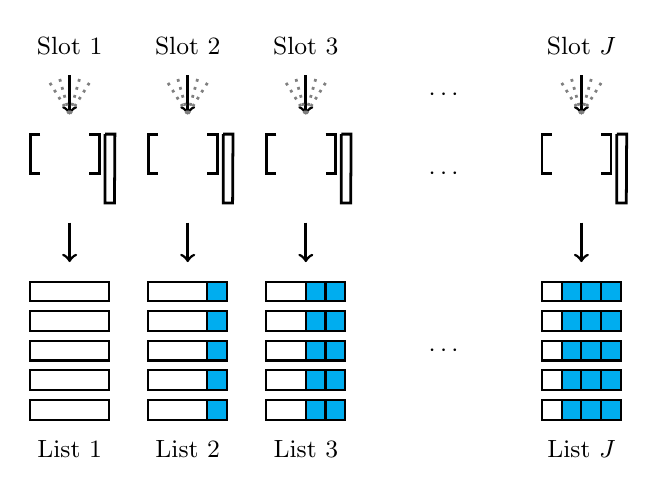
\begin{tikzpicture}
[font=\small, draw=black, line width=0.75pt,
sub0/.style={rectangle, draw, inner sep=0pt, minimum width=10mm, minimum height=2.5mm},
parity/.style={rectangle, draw, fill=cyan, inner sep=0pt, minimum size=2.5mm}]

\node (cs1) at (-1.00,6.125) {Slot~1};
\node (cs2) at (0.50,6.125) {Slot~2};
\node (cs3) at (2.00,6.125) {Slot~3};
\node (cs4) at (5.50,6.125) {Slot~$J$};

\foreach \v in {-1.00,0.50,2.00,5.50} {
  \draw[->, line width=1pt]  (\v,3.875) -- (\v,3.375);
  \draw[->, line width=1pt]  (\v,5.75) -- (\v,5.25);
  \draw[dotted, line width=1pt, draw=gray]  (\v-0.25,5.65) -- (\v,5.25);
  \draw[dotted, line width=1pt, draw=gray]  (\v-0.125,5.7) -- (\v,5.25);
  \draw[dotted, line width=1pt, draw=gray]  (\v+0.125,5.7) -- (\v,5.25);
  \draw[dotted, line width=1pt, draw=gray]  (\v+0.25,5.65) -- (\v,5.25);
}

\node (dots1) at (3.75,5.5) {$\cdots$};

\foreach \v in {-1.00,0.50,2.00,5.50} {
  \draw[line width=1pt] (\v-0.375,5) -- (\v-0.5,5) -- (\v-0.5,4.5) -- (\v-0.375,4.5);
  \draw[line width=1pt] (\v+0.25,5) -- (\v+0.375,5) -- (\v+0.375,4.5) -- (\v+0.25,4.5);
  \draw[line width=1pt] (\v+0.45,5) -- (\v+0.45,4.125) -- (\v+0.57,4.125) -- (\v+0.575,5) -- (\v+0.45,5);
}

\node (dots2) at (3.75,4.5) {$\cdots$};
\node (dots3) at (3.75,2.25) {$\cdots$};

\foreach \c in {3.00, 2.625, 2.25, 1.875, 1.5} {
  \node[sub0] (subcs0\c) at (-1.00,\c) {};
  \node[sub0] (subcs2\c) at (0.50,\c) {};
  \node[parity] (parity0\c) at (0.875,\c) {};
  \node[sub0] (subcs3\c) at (2.00,\c) {};
  \node[parity] (parity1\c) at (2.125,\c) {};
  \node[parity] (parity2\c) at (2.375,\c) {};
  \node[sub0] (subcsz\c) at (5.50,\c) {};
  \node[parity] (parity3\c) at (5.375,\c) {};
  \node[parity] (parity4\c) at (5.625,\c) {};
  \node[parity] (parity5\c) at (5.875,\c) {};
}

\node (list1) at (-1.00,1) {List~1};
\node (list2) at (0.50,1) {List~2};
\node (list3) at (2.00,1) {List~3};
\node (list4) at (5.50,1) {List~$J$};
\end{tikzpicture}
}
\vfill
\begin{itemize}
\item $L$ instances of CS problem, each solved with non-negative LS
\item Produces $L$ lists of $K$ decoded sub-packets (with parity)
\item Must piece sub-packets together using tree decoder
\end{itemize}
\end{frame}


\begin{frame}
\frametitle{Coded Compressive Sensing -- Stitching Process}
  \begin{center}
  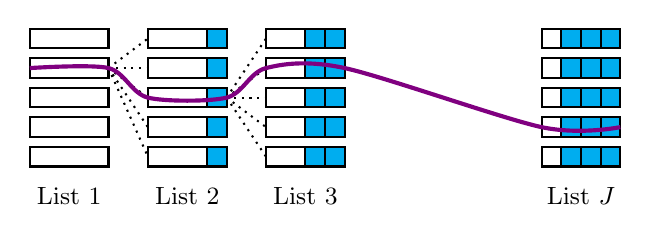
\begin{tikzpicture}
[font=\small, draw=black, line width=0.75pt,
sub0/.style={rectangle, draw, inner sep=0pt, minimum width=10mm, minimum height=2.5mm},
parity/.style={rectangle, draw, fill=cyan, inner sep=0pt, minimum size=2.5mm}]

\foreach \c in {3.00, 2.625, 2.25, 1.875, 1.5} {
  \node[sub0] (subcs1\c) at (-1.00,\c) {};
  \node[sub0] (subcs2\c) at (0.50,\c) {};
  \node[parity] (parity0\c) at (0.875,\c) {};
  \node[sub0] (subcs3\c) at (2.00,\c) {};
  \node[parity] (parity1\c) at (2.125,\c) {};
  \node[parity] (parity2\c) at (2.375,\c) {};
  \node[sub0] (subcsz\c) at (5.50,\c) {};
  \node[parity] (parity3\c) at (5.375,\c) {};
  \node[parity] (parity4\c) at (5.625,\c) {};
  \node[parity] (parity5\c) at (5.875,\c) {};
}

\draw[dotted] (-0.50,2.625) -- (0.00,3.00) {};
\draw[dotted] (-0.50,2.625) -- (0.00,2.625) {};
\draw[dotted] (-0.50,2.625) -- (0.00,2.25) {};
\draw[dotted] (-0.50,2.625) -- (0.00,1.875) {};
\draw[dotted] (-0.50,2.625) -- (0.00,1.50) {};

\draw[dotted] (1.00,2.25) -- (1.50,3.00) {};
\draw[dotted] (1.00,2.25) -- (1.50,2.625) {};
\draw[dotted] (1.00,2.25) -- (1.50,2.25) {};
\draw[dotted] (1.00,2.25) -- (1.50,1.875) {};
\draw[dotted] (1.00,2.25) -- (1.50,1.50) {};

\node (list1) at (-1.00,1) {List~1};
\node (list2) at (0.50,1) {List~2};
\node (list3) at (2.00,1) {List~3};
\node (list4) at (5.50,1) {List~$J$};

\draw [line width=1.5pt,color=violet] plot[smooth, tension=.5] coordinates {
(-1.50,2.625) (-0.50,2.625)
(0.00,2.25) (1.00,2.25)
(1.50,2.625) (2.50,2.625)
(5.00, 1.875) (6.00, 1.875)};
\end{tikzpicture}

  \end{center}
\begin{columns}
\column{.45\textwidth}
\begin{block}{Tree Decoding Principles}
  \begin{itemize}
  \item Every parity is linear combination of bits in preceding blocks
  \item Late parity bits offer better performance
  \item Early parity bits decrease decoding complexity
  %\item Correct fragment is on list
  \end{itemize}
\end{block}
\column{.45\textwidth}
  \centerline{\scalebox{0.5}{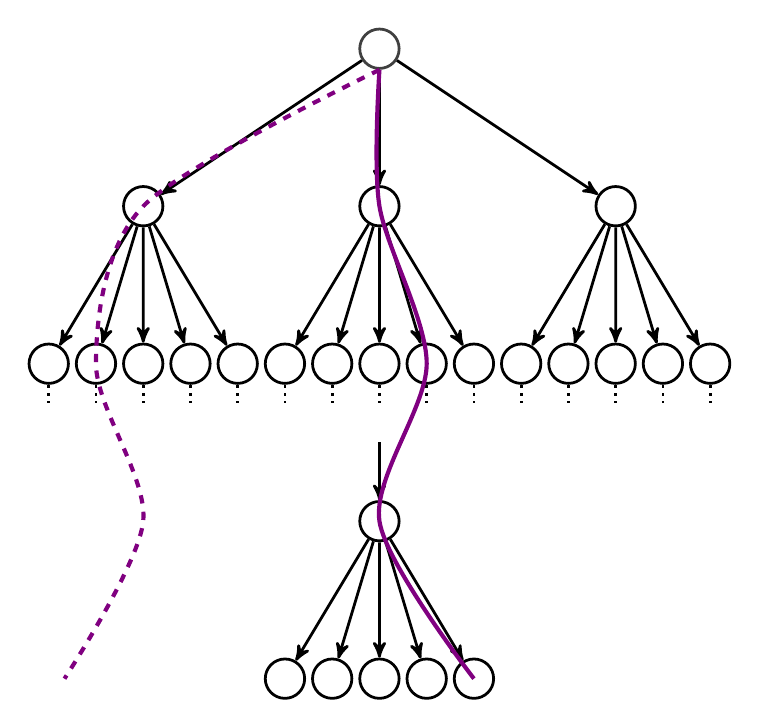
\begin{tikzpicture}
  [
  line width=1pt, draw=black, >=stealth',
  checknode/.style={circle, inner sep=0pt, minimum size=5mm, draw=black}
  ]

  \node[checknode, draw=darkgray] (b1) at (0,4) {};

  \foreach \x in {1,2,3} {
    \node[checknode] (c1\x) at (-6+3*\x,2) {}
      edge[<-] (b1);
  }

  \foreach \y in {1,2,3,4,5} {
    \node[checknode] (b1\y) at (-4.8+0.6*\y,0) {}
      edge[<-] (c11)
      edge[-,dotted] (-4.8+0.6*\y,-0.5);
    \node[checknode] (b2\y) at (-1.8+0.6*\y,0) {}
      edge[<-] (c12)
      edge[-,dotted] (-1.8+0.6*\y,-0.5);
    \node[checknode] (b3\y) at (1.2+0.6*\y,0) {}
      edge[<-] (c13)
      edge[-,dotted] (1.2+0.6*\y,-0.5);
  }
  
  \node[checknode] (c22) at (0,-2) {}
    edge[<-] (0,-1);

  \foreach \y in {1,2,3,4,5} {
    \node[checknode] (b4\y) at (-1.8+0.6*\y,-4) {}
      edge[<-] (c22);
  }

\draw [line width=1.5pt,color=violet] plot[smooth, tension=.5] coordinates {(b1.south) (c12) (b24) (c22) (b45)};
\draw [line width=1.5pt,dashed, color=violet] plot[smooth, tension=.5] coordinates {(b1.south) (c11) (b12) (-3,-2) (-4,-4)};
\end{tikzpicture}
}}
\end{columns}
\end{frame}


\begin{frame}
\frametitle{Extending CCS Framework}
\begin{center}
\begin{tikzpicture}
  \node[scope fading=south] (image) at (0,0) {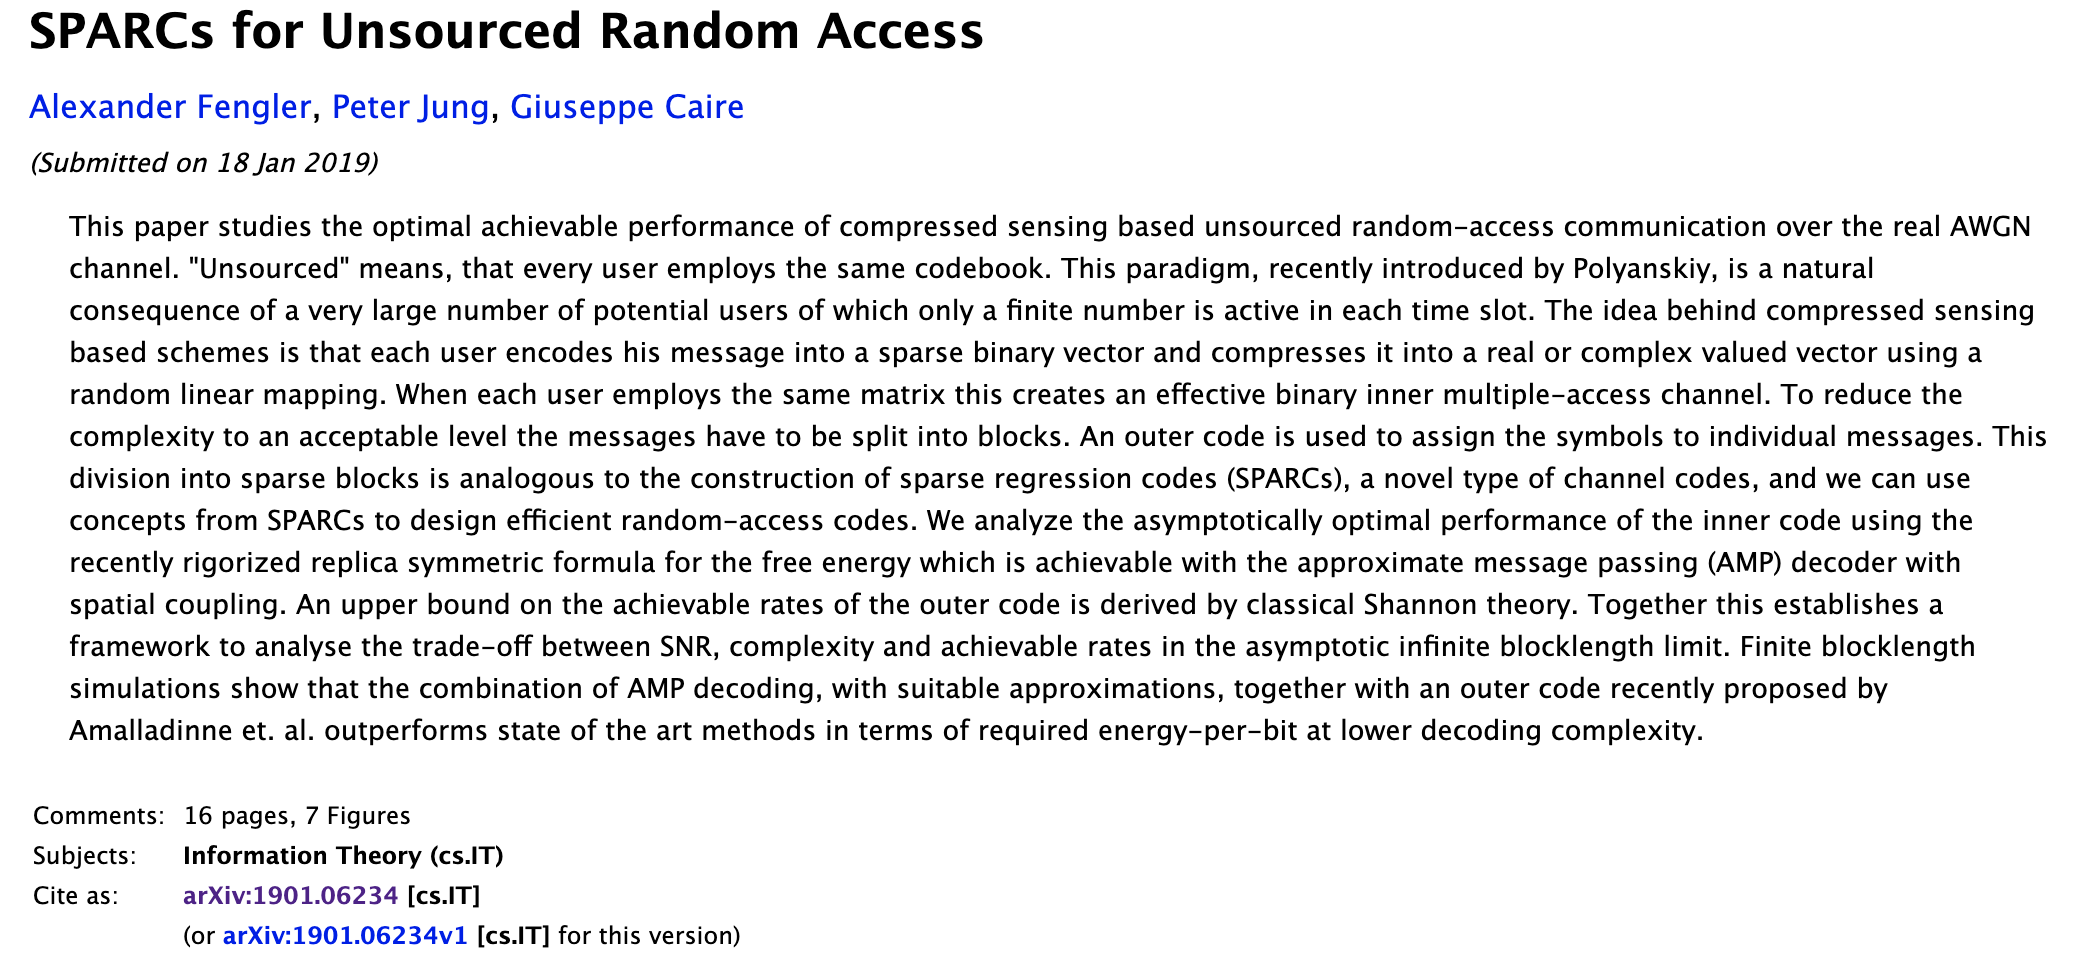
\includegraphics[width=4in]{Figures/SparcsUMAC.png}};
\end{tikzpicture}
\end{center}
  \begin{itemize}
  \item Alexander Fengler, Peter Jung, Giuseppe Caire on arXiv
  \item Connection between CCS indexing and sparse regression codes
  \item Circumvent slotting under CCS and dispersion effects
  \end{itemize}
\end{frame}


\begin{frame}
\frametitle{UMAC -- CCS Revisited}
\begin{center}
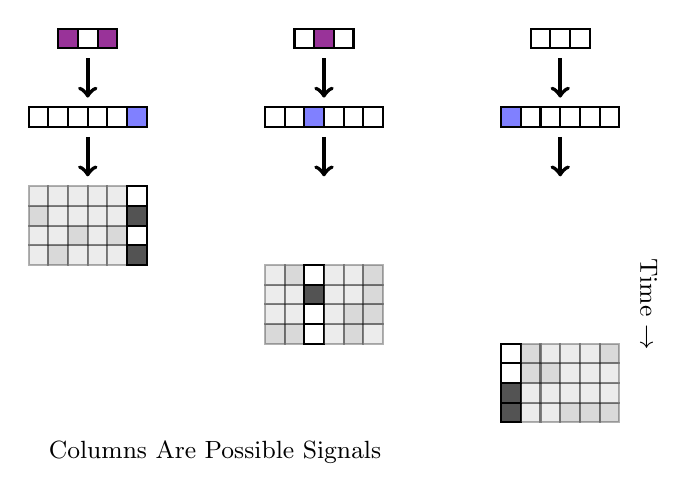
\begin{tikzpicture}
[font=\small, draw=black, line width=0.75pt,
bit0/.style={rectangle, draw, inner sep=0pt, minimum size=2.5mm},
bit1/.style={rectangle, draw, fill=violet!80, inner sep=0pt, minimum size=2.5mm},
entry0/.style={rectangle, draw, opacity=0.3, fill=lightgray, inner sep=0pt, minimum size=2.5mm},
entry1/.style={rectangle, draw, opacity=0.3, fill=gray, inner sep=0pt, minimum size=2.5mm},
entry00/.style={rectangle, draw, fill=white, inner sep=0pt, minimum size=2.5mm},
entry11/.style={rectangle, draw, fill=darkgray!90, inner sep=0pt, minimum size=2.5mm},
symbol0/.style={rectangle, draw, fill=white, inner sep=0pt, minimum size=2.5mm},
symbol1/.style={rectangle, draw, fill=blue!50, inner sep=0pt, minimum size=2.5mm}]

\node[entry11] (m2400) at (6.00,0) {};
\node[entry0] (m2500) at (6.25,0) {};
\node[entry0] (m2600) at (6.50,0) {};
\node[entry1] (m2700) at (6.75,0) {};
\node[entry1] (m2800) at (7.00,0) {};
\node[entry1] (m2900) at (7.25,0) {};

\node[entry11] (m2401) at (6.00,0.25) {};
\node[entry0] (m2501) at (6.25,0.25) {};
\node[entry0] (m2601) at (6.50,0.25) {};
\node[entry0] (m2701) at (6.75,0.25) {};
\node[entry0] (m2801) at (7.00,0.25) {};
\node[entry0] (m2901) at (7.25,0.25) {};

\node[entry00] (m2402) at (6.00,0.50) {};
\node[entry1] (m2502) at (6.25,0.50) {};
\node[entry1] (m2602) at (6.50,0.50) {};
\node[entry0] (m2702) at (6.75,0.50) {};
\node[entry0] (m2802) at (7.00,0.50) {};
\node[entry0] (m2902) at (7.25,0.50) {};

\node[entry00] (m2403) at (6.00,0.75) {};
\node[entry1] (m2503) at (6.25,0.75) {};
\node[entry0] (m2603) at (6.50,0.75) {};
\node[entry0] (m2703) at (6.75,0.75) {};
\node[entry0] (m2803) at (7.00,0.75) {};
\node[entry1] (m2903) at (7.25,0.75) {};

\node[entry1] (m1204) at (3.00,1.00) {};
\node[entry1] (m1304) at (3.25,1.00) {};
\node[entry00] (m1404) at (3.50,1.00) {};
\node[entry0] (m1504) at (3.75,1.00) {};
\node[entry1] (m1604) at (4.00,1.00) {};
\node[entry0] (m1704) at (4.25,1.00) {};

\node[entry0] (m1205) at (3.00,1.25) {};
\node[entry0] (m1305) at (3.25,1.25) {};
\node[entry00] (m1405) at (3.50,1.25) {};
\node[entry0] (m1505) at (3.75,1.25) {};
\node[entry1] (m1605) at (4.00,1.25) {};
\node[entry1] (m1705) at (4.25,1.25) {};

\node[entry0] (m1206) at (3.00,1.50) {};
\node[entry0] (m1306) at (3.25,1.50) {};
\node[entry11] (m1406) at (3.50,1.50) {};
\node[entry0] (m1506) at (3.75,1.50) {};
\node[entry0] (m1606) at (4.00,1.50) {};
\node[entry1] (m1706) at (4.25,1.50) {};

\node[entry0] (m1207) at (3.00,1.75) {};
\node[entry1] (m1307) at (3.25,1.75) {};
\node[entry00] (m1407) at (3.50,1.75) {};
\node[entry0] (m1507) at (3.75,1.75) {};
\node[entry0] (m1607) at (4.00,1.75) {};
\node[entry1] (m1707) at (4.25,1.75) {};

\node[entry0] (m0008) at (0.00,2.00) {};
\node[entry1] (m0108) at (0.25,2.00) {};
\node[entry0] (m0208) at (0.50,2.00) {};
\node[entry0] (m0308) at (0.75,2.00) {};
\node[entry0] (m0408) at (1.00,2.00) {};
\node[entry11] (m0508) at (1.25,2.00) {};

\node[entry0] (m0009) at (0.00,2.25) {};
\node[entry0] (m0109) at (0.25,2.25) {};
\node[entry1] (m0209) at (0.50,2.25) {};
\node[entry0] (m0309) at (0.75,2.25) {};
\node[entry1] (m0409) at (1.00,2.25) {};
\node[entry00] (m0509) at (1.25,2.25) {};

\node[entry1] (m0010) at (0.00,2.50) {};
\node[entry0] (m0110) at (0.25,2.50) {};
\node[entry0] (m0210) at (0.50,2.50) {};
\node[entry0] (m0310) at (0.75,2.50) {};
\node[entry0] (m0410) at (1.00,2.50) {};
\node[entry11] (m0510) at (1.25,2.50) {};

\node[entry0] (m0011) at (0.00,2.75) {};
\node[entry0] (m0111) at (0.25,2.75) {};
\node[entry0] (m0211) at (0.50,2.75) {};
\node[entry0] (m0311) at (0.75,2.75) {};
\node[entry0] (m0411) at (1.00,2.75) {};
\node[entry00] (m0511) at (1.25,2.75) {};

\draw[->, line width=1.5pt]  (0.625,3.50) -- (0.625,3.00);
\draw[->, line width=1.5pt]  (3.625,3.50) -- (3.625,3.00);
\draw[->, line width=1.5pt]  (6.625,3.50) -- (6.625,3.00);

\node[symbol0] (s00) at (0.00,3.75) {};
\node[symbol0] (s01) at (0.25,3.75) {};
\node[symbol0] (s02) at (0.50,3.75) {};
\node[symbol0] (s03) at (0.75,3.75) {};
\node[symbol0] (s04) at (1.00,3.75) {};
\node[symbol1] (s05) at (1.25,3.75) {};

\node[symbol0] (s12) at (3.00,3.75) {};
\node[symbol0] (s13) at (3.25,3.75) {};
\node[symbol1] (s14) at (3.50,3.75) {};
\node[symbol0] (s15) at (3.75,3.75) {};
\node[symbol0] (s16) at (4.00,3.75) {};
\node[symbol0] (s17) at (4.25,3.75) {};

\node[symbol1] (s24) at (6.00,3.75) {};
\node[symbol0] (s25) at (6.25,3.75) {};
\node[symbol0] (s26) at (6.50,3.75) {};
\node[symbol0] (s27) at (6.75,3.75) {};
\node[symbol0] (s28) at (7.00,3.75) {};
\node[symbol0] (s29) at (7.25,3.75) {};

\draw[->, line width=1.5pt]  (0.625,4.50) -- (0.625,4.00);
\draw[->, line width=1.5pt]  (3.625,4.50) -- (3.625,4.00);
\draw[->, line width=1.5pt]  (6.625,4.50) -- (6.625,4.00);

\node[bit1] (info0) at (0.375,4.75) {};
\node[bit0] (info1) at (0.625,4.75) {};
\node[bit1] (info2) at (0.875,4.75) {};
\node[bit0] (info3) at (3.375,4.75) {};
\node[bit1] (info4) at (3.625,4.75) {};
\node[bit0] (info5) at (3.875,4.75) {};
\node[bit0] (info6) at (6.375,4.75) {};
\node[bit0] (info7) at (6.625,4.75) {};
\node[bit0] (info8) at (6.875,4.75) {};


\node [anchor = west] (signals) at (0.00,-0.50) {Columns Are Possible Signals};
\node[rotate=-90] (time) at (7.75,1.375) {Time $\rightarrow$};
\end{tikzpicture}

\end{center}
\begin{itemize}
\item Bit sequence split into $L$ fragments
\item Each bit $+$ parity block converted to index in $[ 1, 2^{M/L} ]$
\item Stack sub-codewords into $(N/L) \times 2^{M/L}$ sensing matrices
\end{itemize}
\end{frame}


\begin{frame}
\frametitle{UMAC -- CCS Unified CS Analogy}
\centerline{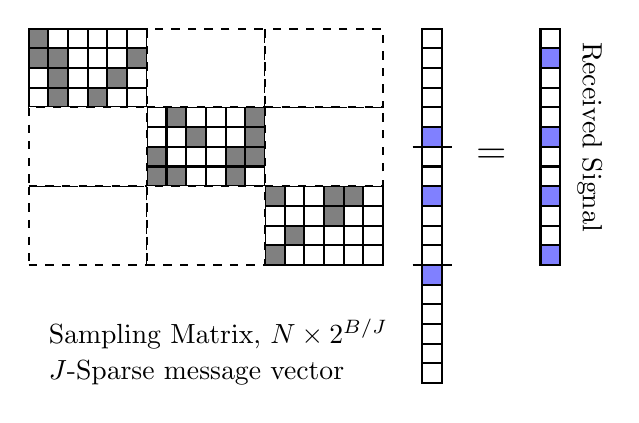
\begin{tikzpicture}
[draw=black, line width=0.75pt,
block/.style={rectangle, draw, fill=white, inner sep=0pt, minimum width=15mm,minimum height=10mm},
entry1/.style={rectangle, draw, fill=gray, inner sep=0pt, minimum size=2.5mm},
entry0/.style={rectangle, draw, fill=white, inner sep=0pt, minimum size=2.5mm},
symbol0/.style={rectangle, draw, fill=white, inner sep=0pt, minimum size=2.5mm},
symbol1/.style={rectangle, draw, fill=blue!50, inner sep=0pt, minimum size=2.5mm}]

\node[entry1] (m1800) at (4.50,0) {};
\node[entry0] (m1900) at (4.75,0) {};
\node[entry0] (m2000) at (5.00,0) {};
\node[entry0] (m2100) at (5.25,0) {};
\node[entry0] (m2200) at (5.50,0) {};
\node[entry0] (m2300) at (5.75,0) {};

\node[entry0] (m1801) at (4.50,0.25) {};
\node[entry1] (m1901) at (4.75,0.25) {};
\node[entry0] (m2001) at (5.00,0.25) {};
\node[entry0] (m2101) at (5.25,0.25) {};
\node[entry0] (m2201) at (5.50,0.25) {};
\node[entry0] (m2301) at (5.75,0.25) {};

\node[entry0] (m1802) at (4.50,0.50) {};
\node[entry0] (m1902) at (4.75,0.50) {};
\node[entry0] (m2002) at (5.00,0.50) {};
\node[entry1] (m2102) at (5.25,0.50) {};
\node[entry0] (m2202) at (5.50,0.50) {};
\node[entry0] (m2302) at (5.75,0.50) {};

\node[entry1] (m1803) at (4.50,0.75) {};
\node[entry0] (m1903) at (4.75,0.75) {};
\node[entry0] (m2003) at (5.00,0.75) {};
\node[entry1] (m2103) at (5.25,0.75) {};
\node[entry1] (m2203) at (5.50,0.75) {};
\node[entry0] (m2303) at (5.75,0.75) {};

\node[entry1] (m1204) at (3.00,1.00) {};
\node[entry1] (m1304) at (3.25,1.00) {};
\node[entry0] (m1404) at (3.50,1.00) {};
\node[entry0] (m1504) at (3.75,1.00) {};
\node[entry1] (m1604) at (4.00,1.00) {};
\node[entry0] (m1704) at (4.25,1.00) {};

\node[entry1] (m1205) at (3.00,1.25) {};
\node[entry0] (m1305) at (3.25,1.25) {};
\node[entry0] (m1405) at (3.50,1.25) {};
\node[entry0] (m1505) at (3.75,1.25) {};
\node[entry1] (m1605) at (4.00,1.25) {};
\node[entry1] (m1705) at (4.25,1.25) {};

\node[entry0] (m1206) at (3.00,1.50) {};
\node[entry0] (m1306) at (3.25,1.50) {};
\node[entry1] (m1406) at (3.50,1.50) {};
\node[entry0] (m1506) at (3.75,1.50) {};
\node[entry0] (m1606) at (4.00,1.50) {};
\node[entry1] (m1706) at (4.25,1.50) {};

\node[entry0] (m1207) at (3.00,1.75) {};
\node[entry1] (m1307) at (3.25,1.75) {};
\node[entry0] (m1407) at (3.50,1.75) {};
\node[entry0] (m1507) at (3.75,1.75) {};
\node[entry0] (m1607) at (4.00,1.75) {};
\node[entry1] (m1707) at (4.25,1.75) {};

\node[entry0] (m0608) at (1.50,2.00) {};
\node[entry1] (m0708) at (1.75,2.00) {};
\node[entry0] (m0808) at (2.00,2.00) {};
\node[entry1] (m0908) at (2.25,2.00) {};
\node[entry0] (m1008) at (2.50,2.00) {};
\node[entry0] (m1108) at (2.75,2.00) {};

\node[entry0] (m0609) at (1.50,2.25) {};
\node[entry1] (m0709) at (1.75,2.25) {};
\node[entry0] (m0809) at (2.00,2.25) {};
\node[entry0] (m0909) at (2.25,2.25) {};
\node[entry1] (m1009) at (2.50,2.25) {};
\node[entry0] (m1109) at (2.75,2.25) {};

\node[entry1] (m0610) at (1.50,2.50) {};
\node[entry1] (m0710) at (1.75,2.50) {};
\node[entry0] (m0810) at (2.00,2.50) {};
\node[entry0] (m0910) at (2.25,2.50) {};
\node[entry0] (m1010) at (2.50,2.50) {};
\node[entry1] (m1110) at (2.75,2.50) {};

\node[entry1] (m0611) at (1.50,2.75) {};
\node[entry0] (m0711) at (1.75,2.75) {};
\node[entry0] (m0811) at (2.00,2.75) {};
\node[entry0] (m0911) at (2.25,2.75) {};
\node[entry0] (m1011) at (2.50,2.75) {};
\node[entry0] (m1111) at (2.75,2.75) {};

\node[block,dashed] at (2.125,0.375) {};
\node[block,dashed] at (2.125,1.375) {};
\node[block,dashed] at (3.625,0.375) {};
\node[block,dashed] at (3.625,2.375) {};
\node[block,dashed] at (5.125,1.375) {};
\node[block,dashed] at (5.125,2.375) {};

\node[symbol0] (s07) at (6.5,-1.50) {};
\node[symbol0] (s08) at (6.5,-1.25) {};
\node[symbol0] (s09) at (6.5,-1.00) {};
\node[symbol0] (s10) at (6.5,-0.75) {};
\node[symbol0] (s11) at (6.5,-0.50) {};
\node[symbol1] (s12) at (6.5,-0.25) {};
\draw (6.25,-0.125) -- (6.75,-0.125);
\node[symbol0] (s13) at (6.5,0) {};
\node[symbol0] (s14) at (6.5,0.25) {};
\node[symbol0] (s15) at (6.5,0.50) {};
\node[symbol1] (s16) at (6.5,0.75) {};
\node[symbol0] (s17) at (6.5,1.00) {};
\node[symbol0] (s18) at (6.5,1.25) {};
\draw (6.25,1.375) -- (6.75,1.375);
\node[symbol1] (s19) at (6.5,1.50) {};
\node[symbol0] (s20) at (6.5,1.75) {};
\node[symbol0] (s21) at (6.5,2.00) {};
\node[symbol0] (s22) at (6.5,2.25) {};
\node[symbol0] (s23) at (6.5,2.50) {};
\node[symbol0] (s24) at (6.5,2.75) {};

\node (equal) at (7.25,1.25) {\Large =};

\node[symbol1] (y00) at (8,0) {};
\node[symbol0] (y01) at (8,0.25) {};
\node[symbol0] (y02) at (8,0.50) {};
\node[symbol1] (y03) at (8,0.75) {};
\node[symbol0] (y04) at (8,1.00) {};
\node[symbol0] (y05) at (8,1.25) {};
\node[symbol1] (y06) at (8,1.50) {};
\node[symbol0] (y07) at (8,1.75) {};
\node[symbol0] (y08) at (8,2.00) {};
\node[symbol0] (y09) at (8,2.25) {};
\node[symbol1] (y10) at (8,2.50) {};
\node[symbol0] (y11) at (8,2.75) {};

\node[anchor=west] (samplingmatrix) at (1.5,-1) {Sampling Matrix, $N \times 2^{{B}/{J}}$};
\node[anchor=west] (vector) at (1.5,-1.5) {$J$-Sparse message vector};
\node[rotate=-90] (receivedsignal) at (8.5,1.5) {Received Signal};
\end{tikzpicture}
}
\begin{itemize}
\item Initial non-linear indexing step
\item Index vector is block sparse
\item Connection to sparse regression codes
\end{itemize}
\myfootnote{\tiny
C. Rush, A. Greig, R. Venkataramanan.
\emph{Capacity-Achieving Sparse Superposition Codes via Approximate Message Passing Decoding}.
IEEE IT Trans 2017}
\end{frame}


\begin{frame}
\frametitle{CCS-AMP}
\centerline{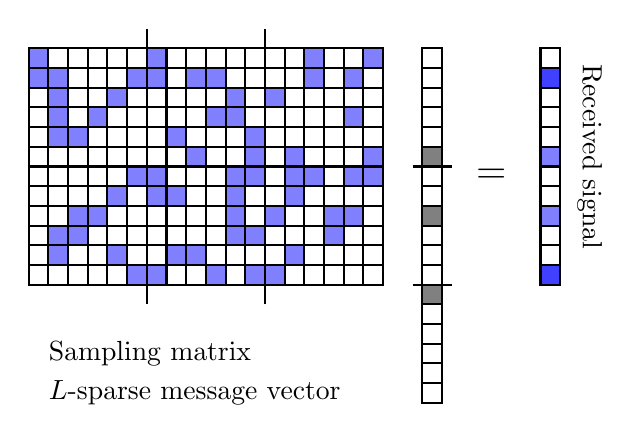
\begin{tikzpicture}
[draw=black, line width=0.75pt,
entry0/.style={rectangle, draw, fill=white, inner sep=0pt, minimum size=2.5mm},
entry1/.style={rectangle, draw, fill=blue!50, inner sep=0pt, minimum size=2.5mm},
symbol0/.style={rectangle, draw, fill=white, inner sep=0pt, minimum size=2.5mm},
symbol1/.style={rectangle, draw, fill=gray, inner sep=0pt, minimum size=2.5mm},
signal0/.style={rectangle, draw, fill=white, inner sep=0pt, minimum size=2.5mm},
signal1/.style={rectangle, draw, fill=blue!50, inner sep=0pt, minimum size=2.5mm},
signal2/.style={rectangle, draw, fill=blue!75, inner sep=0pt, minimum size=2.5mm}]

\node[entry0] (m0600) at (1.50,0) {};
\node[entry0] (m0700) at (1.75,0) {};
\node[entry0] (m0800) at (2.00,0) {};
\node[entry0] (m0900) at (2.25,0) {};
\node[entry0] (m1000) at (2.50,0) {};
\node[entry1] (m1100) at (2.75,0) {};
\node[entry1] (m1200) at (3.00,0) {};
\node[entry0] (m1300) at (3.25,0) {};
\node[entry0] (m1400) at (3.50,0) {};
\node[entry1] (m1500) at (3.75,0) {};
\node[entry0] (m1600) at (4.00,0) {};
\node[entry1] (m1700) at (4.25,0) {};
\node[entry1] (m1800) at (4.50,0) {};
\node[entry0] (m1900) at (4.75,0) {};
\node[entry0] (m2000) at (5.00,0) {};
\node[entry0] (m2100) at (5.25,0) {};
\node[entry0] (m2200) at (5.50,0) {};
\node[entry0] (m2300) at (5.75,0) {};

\node[entry0] (m0601) at (1.50,0.25) {};
\node[entry1] (m0701) at (1.75,0.25) {};
\node[entry0] (m0801) at (2.00,0.25) {};
\node[entry0] (m0901) at (2.25,0.25) {};
\node[entry1] (m1001) at (2.50,0.25) {};
\node[entry0] (m1101) at (2.75,0.25) {};
\node[entry0] (m1201) at (3.00,0.25) {};
\node[entry1] (m1301) at (3.25,0.25) {};
\node[entry1] (m1401) at (3.50,0.25) {};
\node[entry0] (m1501) at (3.75,0.25) {};
\node[entry0] (m1601) at (4.00,0.25) {};
\node[entry0] (m1701) at (4.25,0.25) {};
\node[entry0] (m1801) at (4.50,0.25) {};
\node[entry1] (m1901) at (4.75,0.25) {};
\node[entry0] (m2001) at (5.00,0.25) {};
\node[entry0] (m2101) at (5.25,0.25) {};
\node[entry0] (m2201) at (5.50,0.25) {};
\node[entry0] (m2301) at (5.75,0.25) {};

\node[entry0] (m0602) at (1.50,0.50) {};
\node[entry1] (m0702) at (1.75,0.50) {};
\node[entry1] (m0802) at (2.00,0.50) {};
\node[entry0] (m0902) at (2.25,0.50) {};
\node[entry0] (m1002) at (2.50,0.50) {};
\node[entry0] (m1102) at (2.75,0.50) {};
\node[entry0] (m1202) at (3.00,0.50) {};
\node[entry0] (m1302) at (3.25,0.50) {};
\node[entry0] (m1402) at (3.50,0.50) {};
\node[entry0] (m1502) at (3.75,0.50) {};
\node[entry1] (m1602) at (4.00,0.50) {};
\node[entry1] (m1702) at (4.25,0.50) {};
\node[entry0] (m1802) at (4.50,0.50) {};
\node[entry0] (m1902) at (4.75,0.50) {};
\node[entry0] (m2002) at (5.00,0.50) {};
\node[entry1] (m2102) at (5.25,0.50) {};
\node[entry0] (m2202) at (5.50,0.50) {};
\node[entry0] (m2302) at (5.75,0.50) {};

\node[entry0] (m0603) at (1.50,0.75) {};
\node[entry0] (m0703) at (1.75,0.75) {};
\node[entry1] (m0803) at (2.00,0.75) {};
\node[entry1] (m0903) at (2.25,0.75) {};
\node[entry0] (m1003) at (2.50,0.75) {};
\node[entry0] (m1103) at (2.75,0.75) {};
\node[entry0] (m1203) at (3.00,0.75) {};
\node[entry0] (m1303) at (3.25,0.75) {};
\node[entry0] (m1403) at (3.50,0.75) {};
\node[entry0] (m1503) at (3.75,0.75) {};
\node[entry1] (m1603) at (4.00,0.75) {};
\node[entry0] (m1703) at (4.25,0.75) {};
\node[entry1] (m1803) at (4.50,0.75) {};
\node[entry0] (m1903) at (4.75,0.75) {};
\node[entry0] (m2003) at (5.00,0.75) {};
\node[entry1] (m2103) at (5.25,0.75) {};
\node[entry1] (m2203) at (5.50,0.75) {};
\node[entry0] (m2303) at (5.75,0.75) {};

\node[entry0] (m0604) at (1.50,1.00) {};
\node[entry0] (m0704) at (1.75,1.00) {};
\node[entry0] (m0804) at (2.00,1.00) {};
\node[entry0] (m0904) at (2.25,1.00) {};
\node[entry1] (m1004) at (2.50,1.00) {};
\node[entry0] (m1104) at (2.75,1.00) {};
\node[entry1] (m1204) at (3.00,1.00) {};
\node[entry1] (m1304) at (3.25,1.00) {};
\node[entry0] (m1404) at (3.50,1.00) {};
\node[entry0] (m1504) at (3.75,1.00) {};
\node[entry1] (m1604) at (4.00,1.00) {};
\node[entry0] (m1704) at (4.25,1.00) {};
\node[entry0] (m1804) at (4.50,1.00) {};
\node[entry1] (m1904) at (4.75,1.00) {};
\node[entry0] (m2004) at (5.00,1.00) {};
\node[entry0] (m2104) at (5.25,1.00) {};
\node[entry0] (m2204) at (5.50,1.00) {};
\node[entry0] (m2304) at (5.75,1.00) {};

\node[entry0] (m0605) at (1.50,1.25) {};
\node[entry0] (m0705) at (1.75,1.25) {};
\node[entry0] (m0805) at (2.00,1.25) {};
\node[entry0] (m0905) at (2.25,1.25) {};
\node[entry0] (m1005) at (2.50,1.25) {};
\node[entry1] (m1105) at (2.75,1.25) {};
\node[entry1] (m1205) at (3.00,1.25) {};
\node[entry0] (m1305) at (3.25,1.25) {};
\node[entry0] (m1405) at (3.50,1.25) {};
\node[entry0] (m1505) at (3.75,1.25) {};
\node[entry1] (m1605) at (4.00,1.25) {};
\node[entry1] (m1705) at (4.25,1.25) {};
\node[entry0] (m1805) at (4.50,1.25) {};
\node[entry1] (m1905) at (4.75,1.25) {};
\node[entry1] (m2005) at (5.00,1.25) {};
\node[entry0] (m2105) at (5.25,1.25) {};
\node[entry1] (m2205) at (5.50,1.25) {};
\node[entry1] (m2305) at (5.75,1.25) {};

\node[entry0] (m0606) at (1.50,1.50) {};
\node[entry0] (m0706) at (1.75,1.50) {};
\node[entry0] (m0806) at (2.00,1.50) {};
\node[entry0] (m0906) at (2.25,1.50) {};
\node[entry0] (m1006) at (2.50,1.50) {};
\node[entry0] (m1106) at (2.75,1.50) {};
\node[entry0] (m1206) at (3.00,1.50) {};
\node[entry0] (m1306) at (3.25,1.50) {};
\node[entry1] (m1406) at (3.50,1.50) {};
\node[entry0] (m1506) at (3.75,1.50) {};
\node[entry0] (m1606) at (4.00,1.50) {};
\node[entry1] (m1706) at (4.25,1.50) {};
\node[entry0] (m1806) at (4.50,1.50) {};
\node[entry1] (m1906) at (4.75,1.50) {};
\node[entry0] (m2006) at (5.00,1.50) {};
\node[entry0] (m2106) at (5.25,1.50) {};
\node[entry0] (m2206) at (5.50,1.50) {};
\node[entry1] (m2306) at (5.75,1.50) {};

\node[entry0] (m0607) at (1.50,1.75) {};
\node[entry1] (m0707) at (1.75,1.75) {};
\node[entry1] (m0807) at (2.00,1.75) {};
\node[entry0] (m0907) at (2.25,1.75) {};
\node[entry0] (m1007) at (2.50,1.75) {};
\node[entry0] (m1107) at (2.75,1.75) {};
\node[entry0] (m1207) at (3.00,1.75) {};
\node[entry1] (m1307) at (3.25,1.75) {};
\node[entry0] (m1407) at (3.50,1.75) {};
\node[entry0] (m1507) at (3.75,1.75) {};
\node[entry0] (m1607) at (4.00,1.75) {};
\node[entry1] (m1707) at (4.25,1.75) {};
\node[entry0] (m1807) at (4.50,1.75) {};
\node[entry0] (m1907) at (4.75,1.75) {};
\node[entry0] (m2007) at (5.00,1.75) {};
\node[entry0] (m2107) at (5.25,1.75) {};
\node[entry0] (m2207) at (5.50,1.75) {};
\node[entry0] (m2307) at (5.75,1.75) {};

\node[entry0] (m0608) at (1.50,2.00) {};
\node[entry1] (m0708) at (1.75,2.00) {};
\node[entry0] (m0808) at (2.00,2.00) {};
\node[entry1] (m0908) at (2.25,2.00) {};
\node[entry0] (m1008) at (2.50,2.00) {};
\node[entry0] (m1108) at (2.75,2.00) {};
\node[entry0] (m1208) at (3.00,2.00) {};
\node[entry0] (m1308) at (3.25,2.00) {};
\node[entry0] (m1408) at (3.50,2.00) {};
\node[entry1] (m1508) at (3.75,2.00) {};
\node[entry1] (m1608) at (4.00,2.00) {};
\node[entry0] (m1708) at (4.25,2.00) {};
\node[entry0] (m1808) at (4.50,2.00) {};
\node[entry0] (m1908) at (4.75,2.00) {};
\node[entry0] (m2008) at (5.00,2.00) {};
\node[entry0] (m2108) at (5.25,2.00) {};
\node[entry1] (m2208) at (5.50,2.00) {};
\node[entry0] (m2308) at (5.75,2.00) {};

\node[entry0] (m0609) at (1.50,2.25) {};
\node[entry1] (m0709) at (1.75,2.25) {};
\node[entry0] (m0809) at (2.00,2.25) {};
\node[entry0] (m0909) at (2.25,2.25) {};
\node[entry1] (m1009) at (2.50,2.25) {};
\node[entry0] (m1109) at (2.75,2.25) {};
\node[entry0] (m1209) at (3.00,2.25) {};
\node[entry0] (m1309) at (3.25,2.25) {};
\node[entry0] (m1409) at (3.50,2.25) {};
\node[entry0] (m1509) at (3.75,2.25) {};
\node[entry1] (m1609) at (4.00,2.25) {};
\node[entry0] (m1709) at (4.25,2.25) {};
\node[entry1] (m1809) at (4.50,2.25) {};
\node[entry0] (m1909) at (4.75,2.25) {};
\node[entry0] (m2009) at (5.00,2.25) {};
\node[entry0] (m2109) at (5.25,2.25) {};
\node[entry0] (m2209) at (5.50,2.25) {};
\node[entry0] (m2309) at (5.75,2.25) {};

\node[entry1] (m0610) at (1.50,2.50) {};
\node[entry1] (m0710) at (1.75,2.50) {};
\node[entry0] (m0810) at (2.00,2.50) {};
\node[entry0] (m0910) at (2.25,2.50) {};
\node[entry0] (m1010) at (2.50,2.50) {};
\node[entry1] (m1110) at (2.75,2.50) {};
\node[entry1] (m1210) at (3.00,2.50) {};
\node[entry0] (m1310) at (3.25,2.50) {};
\node[entry1] (m1410) at (3.50,2.50) {};
\node[entry1] (m1510) at (3.75,2.50) {};
\node[entry0] (m1610) at (4.00,2.50) {};
\node[entry0] (m1710) at (4.25,2.50) {};
\node[entry0] (m1810) at (4.50,2.50) {};
\node[entry0] (m1910) at (4.75,2.50) {};
\node[entry1] (m2010) at (5.00,2.50) {};
\node[entry0] (m2110) at (5.25,2.50) {};
\node[entry1] (m2210) at (5.50,2.50) {};
\node[entry0] (m2310) at (5.75,2.50) {};

\node[entry1] (m0611) at (1.50,2.75) {};
\node[entry0] (m0711) at (1.75,2.75) {};
\node[entry0] (m0811) at (2.00,2.75) {};
\node[entry0] (m0911) at (2.25,2.75) {};
\node[entry0] (m1011) at (2.50,2.75) {};
\node[entry0] (m1111) at (2.75,2.75) {};
\node[entry1] (m1211) at (3.00,2.75) {};
\node[entry0] (m1311) at (3.25,2.75) {};
\node[entry0] (m1411) at (3.50,2.75) {};
\node[entry0] (m1511) at (3.75,2.75) {};
\node[entry0] (m1611) at (4.00,2.75) {};
\node[entry0] (m1711) at (4.25,2.75) {};
\node[entry0] (m1811) at (4.50,2.75) {};
\node[entry0] (m1911) at (4.75,2.75) {};
\node[entry1] (m2011) at (5.00,2.75) {};
\node[entry0] (m2111) at (5.25,2.75) {};
\node[entry0] (m2211) at (5.50,2.75) {};
\node[entry1] (m2311) at (5.75,2.75) {};

\draw (2.875,-0.375) -- (2.875,3.125);
\draw (4.375,-0.375) -- (4.375,3.125);

\node[symbol0] (s07) at (6.5,-1.50) {};
\node[symbol0] (s08) at (6.5,-1.25) {};
\node[symbol0] (s09) at (6.5,-1.00) {};
\node[symbol0] (s10) at (6.5,-0.75) {};
\node[symbol0] (s11) at (6.5,-0.50) {};
\node[symbol1] (s12) at (6.5,-0.25) {};
\draw (6.25,-0.125) -- (6.75,-0.125);
\node[symbol0] (s13) at (6.5,0) {};
\node[symbol0] (s14) at (6.5,0.25) {};
\node[symbol0] (s15) at (6.5,0.50) {};
\node[symbol1] (s16) at (6.5,0.75) {};
\node[symbol0] (s17) at (6.5,1.00) {};
\node[symbol0] (s18) at (6.5,1.25) {};
\draw (6.25,1.375) -- (6.75,1.375);
\node[symbol1] (s19) at (6.5,1.50) {};
\node[symbol0] (s20) at (6.5,1.75) {};
\node[symbol0] (s21) at (6.5,2.00) {};
\node[symbol0] (s22) at (6.5,2.25) {};
\node[symbol0] (s23) at (6.5,2.50) {};
\node[symbol0] (s24) at (6.5,2.75) {};

\node (equal) at (7.25,1.25) {\Large =};

\node[signal2] (y00) at (8,0) {};
\node[signal0] (y01) at (8,0.25) {};
\node[signal0] (y02) at (8,0.50) {};
\node[signal1] (y03) at (8,0.75) {};
\node[signal0] (y04) at (8,1.00) {};
\node[signal0] (y05) at (8,1.25) {};
\node[signal1] (y06) at (8,1.50) {};
\node[signal0] (y07) at (8,1.75) {};
\node[signal0] (y08) at (8,2.00) {};
\node[signal0] (y09) at (8,2.25) {};
\node[signal2] (y10) at (8,2.50) {};
\node[signal0] (y11) at (8,2.75) {};

\node[anchor=west] (samplingmatrix) at (1.5,-1) {Sampling matrix};
\node[anchor=west] (vector) at (1.5,-1.5) {$L$-sparse message vector};
\node[rotate=-90] (receivedsignal) at (8.5,1.5) {Received signal};
\end{tikzpicture}
}
\begin{itemize}
\item Complexity management comes from dimensionality reduction
\item Use full sensing matrix on sparse regression codes
\item Decode inner code with low-complexity AMP
\item Decode outer code with tree decoding
\end{itemize}
\myfootnote{\tiny
A. Fengler, P. Jung, and G. Caire.
\emph{SPARCs and AMP for Unsourced Random Access}.
ISIT 2019}
\end{frame}

\begin{frame}
\frametitle{Approximate Message Passing Algorithm}
\begin{block}{Governing Equations}
\begin{itemize}
\item AMP algorithm iterates through
\begin{align*}
\mathbf{z}^{(t)} &= \mathbf{y} - \mathbf{A} \mathbf{D} \boldsymbol{\eta}_t \left( \mathbf{r}^{(t)} \right)
+ \underbrace{\frac{\mathbf{z}^{(t-1)}}{n} \operatorname{div} \mathbf{D} \boldsymbol{\eta}_t \left( \mathbf{r}^{(t)} \right)}_{\text{Onsager correction}} \\
\mathbf{r}^{(t+1)} &= \mathbf{A}^{\mathrm{T}} \mathbf{z}^{(t)} + \mathbf{D}
\underbrace{\boldsymbol{\eta}_t \left( \mathbf{r}^{(t)} \right)}_{\text{Denoiser}}
\end{align*}
\textcolor{gray}{Initial conditions $\mathbf{z}^{(0)} = \mathbf{0}$ and $\boldsymbol{\eta}_0 \left( \mathbf{r}^{(0)} \right) = \mathbf{0}$}
\item Application falls within framework for non-separable functions
\end{itemize}
\end{block}
\begin{exampleblock}{Tasks}
\begin{columns}
\column{.30\textwidth}
\begin{itemize}
\item Define denoiser
\end{itemize}
\column{.60\textwidth}
\begin{itemize}
\item Derive correction term
\end{itemize}
\end{columns}
\end{exampleblock}
\myfootnote{\tiny
R. Berthier, A. Montanari, and P.-M. Nguyen.
\emph{State Evolution for Approximate Message Passing with Non-Separable Functions}.
arXiv 2017}
\end{frame}


\begin{frame}
\frametitle{Marginal Posterior Mean Estimate (PME)}
\begin{block}{Proposed Denoiser (Fengler, Jung, and Caire)}
\begin{itemize}
\item State estimate based on Gaussian model
\begin{equation*}
\begin{split}
\hat{s}^{\mathrm{OR}} & \left( q, r, \tau \right)
= \mathbb{E} \left[ s | \sqrt{P_{\ell}} s + \tau \zeta = r \right] \\
%&= \frac{0 \cdot \Pr (s = 0) f \left( \frac{r}{\tau} \right) + 1 \cdot \Pr (s = 1) f \left( \frac{r - d_{\ell}}{\tau} \right)}{\Pr (s = 0) f \left( \frac{r}{\tau} \right) + \Pr (s = 1) f \left( \frac{r - d_{\ell}}{\tau} \right)} \\
&= \textstyle \frac{q \exp \left( - \frac{ \left( r - \sqrt{P_{\ell}} \right)^2}{2 \tau^2} \right)}
{(1-q) \exp \left( -\frac{r^2}{2 \tau^2} \right)
+ q \exp \left( - \frac{ \left( r - \sqrt{P_{\ell}} \right)^2}{2 \tau^2} \right)}
\end{split}
\end{equation*}
with prior $q = K/m$ fixed
\item $\boldsymbol{\eta}_t \left( \mathbf{r}^{(t)} \right)$ is aggregate of PME values
\item $\tau_t$ is obtained from state evolution or $\tau_t^2 = {\| \mathbf{z}^{(t)} \|^2}/{n}$
\end{itemize}
\end{block}
\vfill
\begin{center}
\begin{tikzpicture}
\shade[draw=none,
left color={rgb:red,1;green,2;blue,3},
right color=frametitle.fg,
shading angle=60,
rounded corners,
blur shadow={shadow blur steps=5}] (-3.75,-0.625) rectangle (3.75,0.625);
\shade[fill=white, fill opacity=0.1] (-3.75,-0.625) rectangle (3.75,0.625);
\node at (0,0) {\textcolor{white}{\Large \textbf{
Performance is quite good!
}}};
\end{tikzpicture}
\end{center}
\end{frame}

\begin{frame}
\frametitle{Marginal PME Revisited}
\begin{block}{Enhanced CCS-AMP}
\begin{itemize}
\item Can one use tree structure to inform AMP denoiser?
\item Idea: Propagate beliefs through $q$ within PME exisiting framework
\begin{equation*}
\begin{split}
\hat{s}^{\mathrm{OR}} & \left( q, r, \tau \right)
= \mathbb{E} \left[ s | \sqrt{P_{\ell}} s + \tau \zeta = r \right] \\
&= \textstyle \frac{q \exp \left( - \frac{ \left( r - \sqrt{P_{\ell}} \right)^2}{2 \tau^2} \right)}
{(1-q) \exp \left( -\frac{r^2}{2 \tau^2} \right)
+ q \exp \left( - \frac{ \left( r - \sqrt{P_{\ell}} \right)^2}{2 \tau^2} \right)}
\end{split}
\end{equation*}
but leverage extrinsic information to compute $q = \Pr (s = 1)$
\item Proposed denoiser becomes
\begin{equation*}
\left( \boldsymbol{\eta}_t \left( \mathbf{r} \right) \right)_k
= \hat{s}^{\mathrm{OR}} \left( \left( \mathbf{q} \left( \mathbf{r} \right) \right)_k, \left( \mathbf{r} \right)_k, \tau_t \right)
\end{equation*}
where $( \cdot )_k$ is $k$th component
\end{itemize}
\end{block}
\end{frame}


\begin{frame}
\frametitle{Updated CCS-AMP Equations}
\begin{itemize}
\item Onsager correction from divergence of $\boldsymbol{\eta}_t (\mathbf{r})$
\begin{equation*}
\frac{1}{n} \operatorname{div} \mathbf{D} \boldsymbol{\eta}_t \left( \mathbf{r} \right)
= \frac{1}{n \tau_t^2} \left( K P - \left\| \mathbf{D} \boldsymbol{\eta}_t \left( \mathbf{r} \right) \right\|^2 \right)
\end{equation*}
\item Robust to tree dynamics
\item Simplified AMP equations
\begin{align*}
\mathbf{z}^{(t)} &= \mathbf{y} - \mathbf{A} \mathbf{D} \mathbf{s}^{(t)} + \frac{\mathbf{z}^{(t-1)}}{n \tau_t^2} \left( K P - \left\| \mathbf{D} \mathbf{s}^{(t)} \right\|^2 \right) \\
\mathbf{s}^{(t+1)} &= \boldsymbol{\eta}_{t+1} \left( \mathbf{A}^{\mathrm{T}} \mathbf{z}^{(t)} + \mathbf{D} \mathbf{s}^{(t)} \right)
\end{align*}
with $\left( \boldsymbol{\eta}_t \left( \mathbf{r} \right) \right)_k = \hat{s}^{\mathrm{OR}} \left( \left( \mathbf{q} \left( \mathbf{r} \right) \right)_k, \left( \mathbf{r} \right)_k, \tau_t \right)$
\end{itemize}
\begin{exampleblock}{Tasks}
\begin{enumerate}
\item Devise a suitable tree code
\item Compute $\mathbf{q} \left( \mathbf{r} \right)$ from tree code
\end{enumerate}
\end{exampleblock}
\end{frame}


\begin{frame}
\frametitle{Redesigning Outer Code}
\begin{block}{Properties of Original Tree Code}
\begin{itemize}
\item Aimed at stitching message fragments together
\item Works on short lists of $K$ fragments
\item Parities allocated to control growth and complexity
\end{itemize}
\end{block}
\centerline{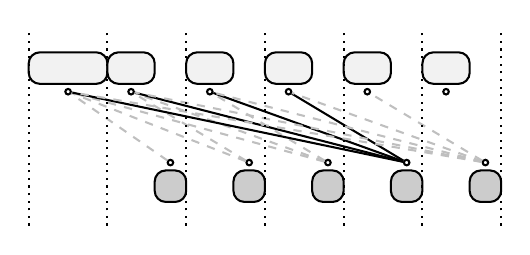
\begin{tikzpicture}[
  font=\footnotesize, >=stealth', line width=0.75pt,
  infobits0/.style={rectangle, minimum height=4mm, minimum width=10mm, draw=black, fill=gray!10, rounded corners},
  infobits/.style={rectangle, minimum height=4mm, minimum width=6mm, draw=black, fill=gray!10, rounded corners},
  paritybits/.style={rectangle, minimum height=4mm, minimum width=4mm, draw=black, fill=gray!40, rounded corners},
  dot/.style={circle, minimum width=2pt, draw=black, inner sep=0pt}
]

\node[infobits0] (vb0) at (0,1.5) {};
\node[infobits] (vb1) at (0.8,1.5) {};
\node[paritybits] (vp1) at (1.3,0) {};
\node[infobits] (vb2) at (1.8,1.5) {};
\node[paritybits] (vp2) at (2.3,0) {};
\node[infobits] (vb3) at (2.8,1.5) {};
\node[paritybits] (vp3) at (3.3,0) {};
\node[infobits] (vb4) at (3.8,1.5) {};
\node[paritybits] (vp4) at (4.3,0) {};
\node[infobits] (vb5) at (4.8,1.5) {};
\node[paritybits] (vp5) at (5.3,0) {};

\node[dot] (vb0dot) at (0.0,1.2) {};
\node[dot] (vb1dot) at (0.8,1.2) {};
\node[dot] (vp1dot) at (1.3,0.3) {}
  edge[-,dashed,draw=lightgray] (vb0dot);
\node[dot] (vb2dot) at (1.8,1.2) {};
\node[dot] (vp2dot) at (2.3,0.3) {}
  edge[-,dashed,draw=lightgray] (vb0dot)
  edge[-,dashed,draw=lightgray] (vb1dot);
\node[dot] (vb3dot) at (2.8,1.2) {};
\node[dot] (vp3dot) at (3.3,0.3) {}
  edge[-,dashed,draw=lightgray] (vb0dot)
  edge[-,dashed,draw=lightgray] (vb1dot)
  edge[-,dashed,draw=lightgray] (vb2dot);
\node[dot] (vb4dot) at (3.8,1.2) {};
\node[dot] (vp4dot) at (4.3,0.3) {}
  edge[-] (vb0dot)
  edge[-] (vb1dot)
  edge[-] (vb2dot)
  edge[-] (vb3dot);
\node[dot] (vb5dot) at (4.8,1.2) {};
\node[dot] (vp5dot) at (5.3,0.3) {}
  edge[-,dashed,draw=lightgray] (vb0dot)
  edge[-,dashed,draw=lightgray] (vb1dot)
  edge[-,dashed,draw=lightgray] (vb2dot)
  edge[-,dashed,draw=lightgray] (vb3dot)
  edge[-,dashed,draw=lightgray] (vb4dot);

\foreach \x in {-0.5,0.5,1.5,2.5,3.5,4.5,5.5} {
    \draw[dotted] (\x,-0.5) -- (\x,2);
}
\end{tikzpicture}
}
\begin{block}{Challenges to Integrate into AMP}
\begin{enumerate}
\item Must compute beliefs for all possible $2^v$ fragments
\item Must provide pertinent information to AMP
\item Should maintain ability to stitch outer code
\end{enumerate}
\end{block}
\end{frame}


\begin{frame}
\frametitle{Redesigning Outer Code}
\begin{block}{Solutions to Integrate into AMP}
\begin{itemize}
\item Parity bits are generated over Abelian group amenable to\\
Hadamard transform (original) or FFT (modified)
\item Discrimination power proportional to \# parities
\end{itemize}
\end{block}
\centerline{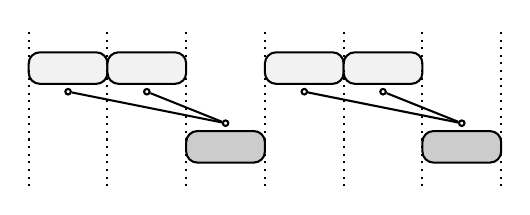
\begin{tikzpicture}[
  font=\footnotesize, >=stealth', line width=0.75pt,
  infobits/.style={rectangle, minimum height=4mm, minimum width=10mm, draw=black, fill=gray!10, rounded corners},
  paritybits/.style={rectangle, minimum height=4mm, minimum width=10mm, draw=black, fill=gray!40, rounded corners},
  dot/.style={circle, minimum width=2pt, draw=black, inner sep=0pt}
]

\node[infobits] (vb0) at (0,1) {};
\node[infobits] (vb1) at (1,1) {};
\node[paritybits] (vp2) at (2,0) {};
\node[infobits] (vb3) at (3,1) {};
\node[infobits] (vb4) at (4,1) {};
\node[paritybits] (vp5) at (5,0) {};

\node[dot] (vb0dot) at (0,0.7) {};
\node[dot] (vb1dot) at (1,0.7) {};
\node[dot] (vp2dot) at (2,0.3) {}
  edge[-] (vb0dot)
  edge[-] (vb1dot);
\node[dot] (vb3dot) at (3,0.7) {};
\node[dot] (vb4dot) at (4,0.7) {};
\node[dot] (vp5dot) at (5,0.3) {}
  edge[-] (vb3dot)
  edge[-] (vb4dot);

\foreach \x in {-0.5,0.5,1.5,2.5,3.5,4.5,5.5} {
    \draw[dotted] (\x,-0.5) -- (\x,1.5);
}
\end{tikzpicture}
}
\begin{block}{New Design Strategy}
\begin{enumerate}
\item Information sections with parity bits interspersed in-between
\item Parity over two blocks (triadic dependencies)
\item Multiplicative effect across concentrated sections
\end{enumerate}
\end{block}
\end{frame}


\begin{frame}
\frametitle{Redesigning Outer Code}
\begin{itemize}
\item Circular convolution structure
\begin{equation*}
\text{Extrinsic Info }
\left( \mathbf{q}(\ell) \right)_k
\textstyle \propto \sum_{\{ g_j \}, \sum_{j} g_j \equiv k} \left( \prod_{j}
\mathcal{L}_{j} \left( \hat{\mathbf{s}}(j) \right) \right)
\end{equation*}
where $\hat{\mathbf{s}}(j) \in \mathbf{G}_{j,\ell}^{-1}(g_j)$.
\item Fast transform techniques
\begin{equation*}
\text{Extrinsic Info Vector }
\mathbf{q}(\ell)
\textstyle \propto \operatorname{FFT}^{-1} \left( \prod_{j} \operatorname{FFT} \left( \boldsymbol{\mathcal{L}}_{j,\ell} \right) \right)
\end{equation*}
\end{itemize}
\centerline{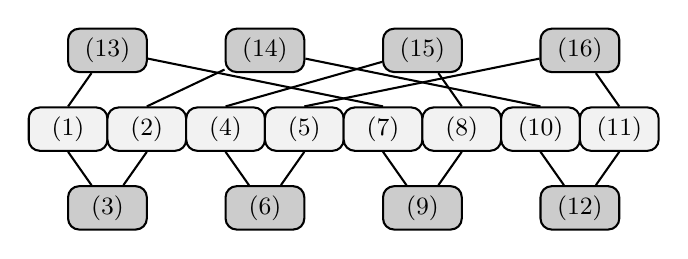
\begin{tikzpicture}[
  font=\small, >=stealth', line width=0.75pt,
  infobits/.style={rectangle, minimum height=3mm, minimum width=10mm, draw=black, fill=gray!10, rounded corners},
  paritybits/.style={rectangle, minimum height=3mm, minimum width=10mm, draw=black, fill=gray!40, rounded corners}
]

\node[infobits] (vb1) at (1,0) {$\vv(1)$};
\node[infobits] (vb2) at (2,0) {$\vv(2)$};
\node[infobits] (vb4) at (3,0) {$\vv(4)$};
\node[infobits] (vb5) at (4,0) {$\vv(5)$};
\node[infobits] (vb7) at (5,0) {$\vv(7)$};
\node[infobits] (vb8) at (6,0) {$\vv(8)$};
\node[infobits] (vb10) at (7,0) {$\vv(10)$};
\node[infobits] (vb11) at (8,0) {$\vv(11)$};

\node[paritybits] (vp3) at (1.5,-1) {$\vv(3)$};
\node[paritybits] (vp6) at (3.5,-1) {$\vv(6)$};
\node[paritybits] (vp9) at (5.5,-1) {$\vv(9)$};
\node[paritybits] (vp12) at (7.5,-1) {$\vv(12)$};
\node[paritybits] (vp13) at (1.5,1) {$\vv(13)$};
\node[paritybits] (vp14) at (3.5,1) {$\vv(14)$};
\node[paritybits] (vp15) at (5.5,1) {$\vv(15)$};

\node[paritybits] (vp16) at (7.5,1) {$\vv(16)$};

\draw  (vb1.south) edge (vp3);
\draw  (vb2.south) edge (vp3);
\draw  (vb4.south) edge (vp6);
\draw  (vb5.south) edge (vp6);
\draw  (vb7.south) edge (vp9);
\draw  (vb8.south) edge (vp9);
\draw  (vb10.south) edge (vp12);
\draw  (vb11.south) edge (vp12);

\draw  (vb1.north) edge (vp13);
\draw  (vb7.north) edge (vp13);
\draw  (vb2.north) edge (vp14);
\draw  (vb10.north) edge (vp14);
\draw  (vb4.north) edge (vp15);
\draw  (vb8.north) edge (vp15);
\draw  (vb5.north) edge (vp16);
\draw  (vb11.north) edge (vp16);

\end{tikzpicture}
}
\end{frame}


\begin{frame}
\frametitle{Preliminary Performance Enhanced CCS}
\centerline{
  \scalebox{0.65}{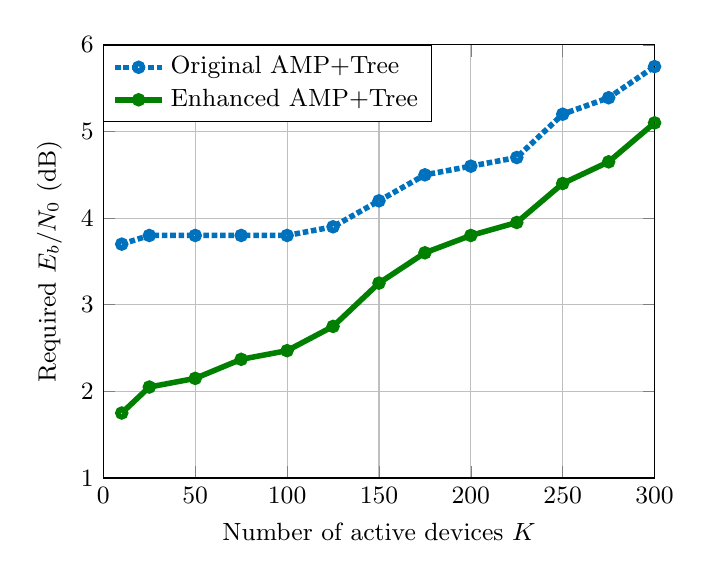
\begin{tikzpicture}
\definecolor{mycolor1}{rgb}{0.63529,0.07843,0.18431}%
\definecolor{mycolor2}{rgb}{0.00000,0.44706,0.74118}%
\definecolor{mycolor3}{rgb}{0.00000,0.49804,0.00000}%
\definecolor{mycolor4}{rgb}{0.87059,0.49020,0.00000}%
\definecolor{mycolor5}{rgb}{0.00000,0.44700,0.74100}%
\definecolor{mycolor6}{rgb}{0.74902,0.00000,0.74902}%

\begin{axis}[%
font=\small,
width=7cm,
height=5.5cm,
scale only axis,
xmin=0,
xmax=300,
xtick = {0,50,100,...,300},
xlabel={Number of active devices $K$},
xmajorgrids,
ymin=1,
ymax=6,
ytick = {1,...,6},
ylabel={Required $E_b/N_0$ (dB)},
ymajorgrids,
legend style={at={(0,1)},anchor=north west, draw=black,fill=white,legend cell align=left}
]



\addplot [color=mycolor2,densely dotted,line width=2.0pt,mark size=1.4pt,mark=o, mark options={solid}]
  table[row sep=crcr]{10 3.7\\
25	3.8\\
50	3.8\\
75	3.8\\
100	3.8\\
125	3.9\\
150	4.2\\
175 4.5\\
200 4.6\\
225 4.7\\
250 5.2\\
275 5.39\\
300 5.75\\
};
\addlegendentry{Original AMP+Tree};

\addplot [color=mycolor3,solid,line width=2.0pt,mark size=1.4pt,mark=o,mark options={solid}]
  table[row sep=crcr]{10 1.75\\
  25  2.05\\
50	2.15\\
75	2.37\\
100	2.47\\
125	2.75\\
150	3.25\\
175 3.6\\
200 3.8\\
225 3.95\\
250 4.4\\
275 4.65\\
300 5.1\\
};
\addlegendentry{Enhanced AMP+Tree};

%\addplot [color=mycolor1,densely dashdotted,line width=2.0pt,mark size=1.4pt,mark=square,mark options={solid}]
%  table[row sep=crcr]{
%  25  2\\
%50	2.1\\
%75	2.2\\
%100	2.41\\
%125	2.57\\
%150	2.81\\
%175	3\\
%200 3.4\\
%225 3.88\\
%250 4.36\\
%275 4.87\\
%300 5.35\\
%};
%\addlegendentry{Sparse IDMA};


\end{axis}


\end{tikzpicture}
}
  \scalebox{0.65}{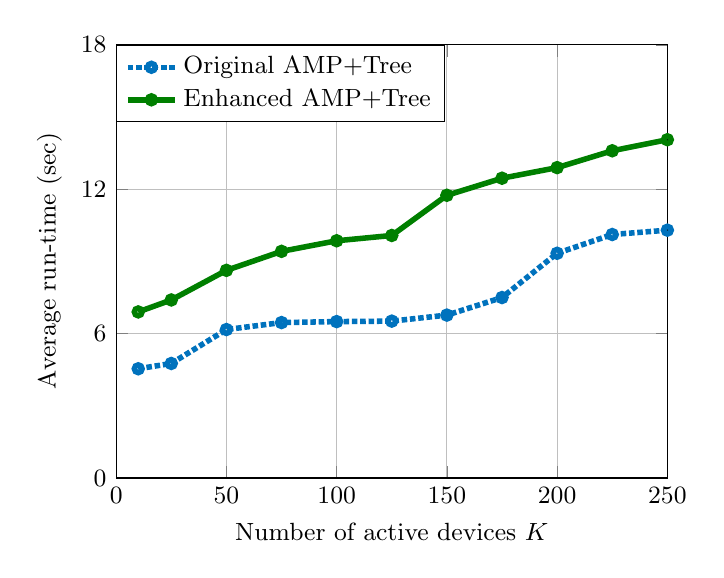
\begin{tikzpicture}
\definecolor{mycolor1}{rgb}{0.63529,0.07843,0.18431}%
\definecolor{mycolor2}{rgb}{0.00000,0.44706,0.74118}%
\definecolor{mycolor3}{rgb}{0.00000,0.49804,0.00000}%
\definecolor{mycolor4}{rgb}{0.87059,0.49020,0.00000}%
\definecolor{mycolor5}{rgb}{0.00000,0.44700,0.74100}%
\definecolor{mycolor6}{rgb}{0.74902,0.00000,0.74902}%

\begin{axis}[%
font=\small,
width=7cm,
height=5.5cm,
scale only axis,
xmin=0,
xmax=250,
xtick = {0,50,100,...,250},
xlabel={Number of active devices $K$},
xmajorgrids,
ymin=0,
ymax=18,
ytick = {0,6,...,18},
ylabel={Average run-time (sec)},
ymajorgrids,
legend style={at={(0,1)},anchor=north west, draw=black,fill=white,legend cell align=left}
]


\addplot [color=mycolor2,densely dotted,line width=2.0pt,mark size=1.4pt,mark=o, mark options={solid}]
  table[row sep=crcr]{10 4.54\\
25	4.76\\
50	6.17\\
75	6.46\\
100	6.5\\
125	6.52\\
150	6.77\\
175 7.5\\
200 9.34\\
225 10.12\\
250 10.3\\
};
\addlegendentry{Original AMP+Tree};

\addplot [color=mycolor3,solid,line width=2.0pt,mark size=1.4pt,mark=o,mark options={solid}]
  table[row sep=crcr]{10 6.903\\
  25  7.4\\
50	8.63\\
75	9.42\\
100	9.86\\
125	10.08\\
150 11.75\\
175 12.46\\
200 12.9\\
225 13.6\\
250 14.06\\
};
\addlegendentry{Enhanced AMP+Tree};
\end{axis}

\end{tikzpicture}
}}
\vspace{5mm}
\begin{itemize}
\item Overall performance improves significantly with enhanced CCS-AMP decoding
\item Computational complexity is approximately maintained
\item Reparametrization may offer additional gains in performance?
\end{itemize}
\end{frame}


\begin{frame}
\frametitle{Discussion -- Unsourced Multiple Access Channel}
\begin{block}{Summary}
\begin{itemize}
\item Introduced new framework for CCS-AMP and unsourced multiple access
\item There are close connections between compressive sensing, graph-based codes, and UMAC
\item Many theoretical and practical challenges/opportunities exist
\end{itemize}
\end{block}
\vspace{5mm}
\begin{center}
  \begin{tikzpicture}
  \shade[draw=none,
  left color={rgb:red,1;green,2;blue,3},
  right color=frametitle.fg,
  shading angle=60,
  rounded corners,
  blur shadow={shadow blur steps=5}] (-2.25,-0.625) rectangle (2.25,0.625);
  \shade[fill=white, fill opacity=0.1] (-2.25,-0.625) rectangle (2.25,0.625);
  \node at (0,0) {\textcolor{white}{\Large \textbf{Questions?}}};
  \end{tikzpicture}
\end{center}
\end{frame}


\begin{frame}
  \begin{center}
  \begin{tikzpicture}
  \shade[draw=none,
  left color={rgb:red,1;green,2;blue,3},
  right color=frametitle.fg,
  shading angle=60,
  rounded corners,
  blur shadow={shadow blur steps=5}] (-2.25,-0.625) rectangle (2.25,0.625);
  \shade[fill=white, fill opacity=0.1] (-2.25,-0.625) rectangle (2.25,0.625);
  \node at (0,0) {\textcolor{white}{\Large \textbf{Thank You!}}};
  \end{tikzpicture}
  \end{center}
\vfill
\begin{center}
\scalebox{0.75}{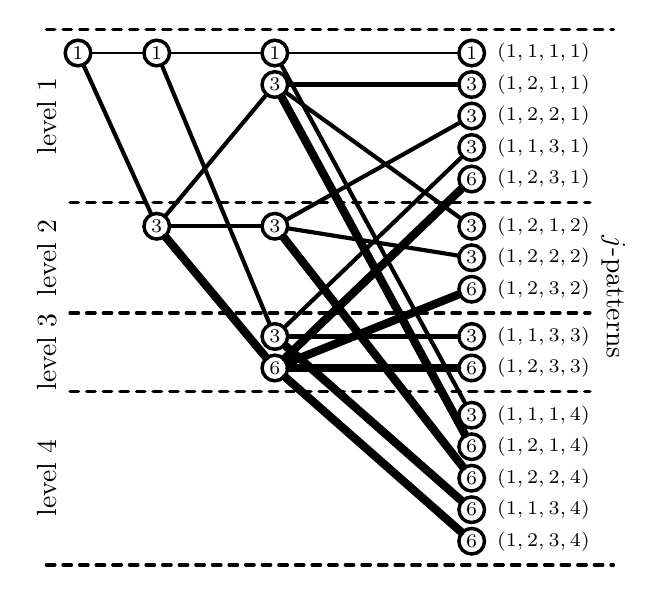
\begin{tikzpicture}[
  font=\scriptsize, >=stealth', line width=1.25pt, line cap=round,
  node/.style={circle, minimum size=3.25mm, inner sep=0pt, draw=black}
]

\node[node] (s1) at (0,3.1) {1};
  \node[node] (s1-1) at (1,3.1) {1};
    \node[node] (s1-1-1) at (2.5,3.1) {1};
      \node[node,label=right:{$(1,1,1,1)$}] (s1-1-1-1) at (5,3.1) {1};
      \node[node,label=right:{$(1,1,1,4)$}] (s1-1-1-4) at (5,-1.5) {3};
    \node[node] (s1-1-3) at (2.5,-0.5) {3};
      \node[node,label=right:{$(1,1,3,1)$}] (s1-1-3-1) at (5,1.9) {3};
      \node[node,label=right:{$(1,1,3,3)$}] (s1-1-3-3) at (5,-0.5) {3};
      \node[node,label=right:{$(1,1,3,4)$}] (s1-1-3-4) at (5,-2.7) {6};
  \node[node] (s1-2) at (1,0.9) {3};
    \node[node] (s1-2-1) at (2.5,2.7) {3};
      \node[node,label=right:{$(1,2,1,1)$}] (s1-2-1-1) at (5,2.7) {3};
      \node[node,label=right:{$(1,2,1,2)$}] (s1-2-1-2) at (5,0.9) {3};
      \node[node,label=right:{$(1,2,1,4)$}] (s1-2-1-4) at (5,-1.9) {6};
    \node[node] (s1-2-2) at (2.5,0.9) {3};
      \node[node,label=right:{$(1,2,2,1)$}] (s1-2-2-1) at (5,2.3) {3};
      \node[node,label=right:{$(1,2,2,2)$}] (s1-2-2-2) at (5,0.5) {3};
      \node[node,label=right:{$(1,2,2,4)$}] (s1-2-2-4) at (5,-2.3) {6};
    \node[node] (s1-2-3) at (2.5,-0.9) {6};
      \node[node,label=right:{$(1,2,3,1)$}] (s1-2-3-1) at (5,1.5) {6};
      \node[node,label=right:{$(1,2,3,2)$}] (s1-2-3-2) at (5,0.1) {6};
      \node[node,label=right:{$(1,2,3,3)$}] (s1-2-3-3) at (5,-0.9) {6};
      \node[node,label=right:{$(1,2,3,4)$}] (s1-2-3-4) at (5,-3.1) {6};

\draw[line width=0.5pt] (s1) -- (s1-1);
  \draw[line width=0.5pt] (s1-1) -- (s1-1-1);
    \draw[line width=0.5pt] (s1-1-1) -- (s1-1-1-1);
    \draw[line width=1.5pt] (s1-1-1) -- (s1-1-1-4);
  \draw[line width=1.5pt] (s1-1) -- (s1-1-3);
    \draw[line width=1.5pt] (s1-1-3) -- (s1-1-3-1);
    \draw[line width=1.5pt] (s1-1-3) -- (s1-1-3-3);
    \draw[line width=3.0pt] (s1-1-3) -- (s1-1-3-4);
\draw[line width=1.5pt] (s1) -- (s1-2);
  \draw[line width=1.5pt] (s1-2) -- (s1-2-1);
    \draw[line width=1.5pt] (s1-2-1) -- (s1-2-1-1);
    \draw[line width=1.5pt] (s1-2-1) -- (s1-2-1-2);
    \draw[line width=3.0pt] (s1-2-1) -- (s1-2-1-4);
  \draw[line width=1.5pt] (s1-2) -- (s1-2-2);
    \draw[line width=1.5pt] (s1-2-2) -- (s1-2-2-1);
    \draw[line width=1.5pt] (s1-2-2) -- (s1-2-2-2);
    \draw[line width=3.0pt] (s1-2-2) -- (s1-2-2-4);
  \draw[line width=3.0pt] (s1-2) -- (s1-2-3);
    \draw[line width=3.0pt] (s1-2-3) -- (s1-2-3-1);
    \draw[line width=3.0pt] (s1-2-3) -- (s1-2-3-2);
    \draw[line width=3.0pt] (s1-2-3) -- (s1-2-3-3);
    \draw[line width=3.0pt] (s1-2-3) -- (s1-2-3-4);

\draw[dashed] (-0.4,3.4) -- (6.8,3.4);
\draw[dashed] (-0.1,1.2) -- (6.5,1.2);
\draw[dashed] (-0.1,-0.2) -- (6.5,-0.2);
\draw[dashed] (-0.1,-1.2) -- (6.5,-1.2);
\draw[dashed] (-0.4,-3.4) -- (6.8,-3.4);

\node[rotate=90] at (-0.4,2.3) {\normalsize level~$1$};
\node[rotate=90] at (-0.4,0.5) {\normalsize level~$2$};
\node[rotate=90] at (-0.4,-0.7) {\normalsize level~$3$};
\node[rotate=90] at (-0.4,-2.3) {\normalsize level~$4$};

\node[rotate=-90] at (6.8,0) {\normalsize $j$-patterns};
\end{tikzpicture}
}
\end{center}
\myfootnote{\scriptsize This material is based upon work supported, in part, by NSF under Grant No.~1619085}
\myfootnote{\scriptsize This material is also based upon work support, in part, by Qualcomm Technologies, Inc., through their University Relations Program}
\end{frame}

\end{document}
